\documentclass[11pt, a4paper]{article} % , draft
\usepackage[utf8]{inputenc}

\usepackage{enumitem} % customiçe item dots etc
\usepackage{textgreek} % obv
\usepackage{physics} % for easy derivative notation
\usepackage{amsmath}
\usepackage{amsthm} %theorems
\usepackage{amssymb}
\usepackage{mathtools} % for matrices with blocks inside
\usepackage[scr=boondoxo]{mathalfa}
\usepackage{pst-node}%
\usepackage{mathrsfs}
\DeclareMathAlphabet{\mathpzc}{OT1}{pzc}{m}{it}

\newcommand{\mc}{\multicolumn{1}{c}}
\newcommand{\R}{\mathbb{R}} % command for real R
\newcommand{\Holo}{\mathcal{H}}
\newcommand{\M}{\mathcal{M}}
\newcommand{\C}{\mathbb{C}}
\newcommand{\N}{\mathbb{N}}
\newcommand{\z}{\mathpzc{s}}
\newcommand{\p}{\mathpzc{r}}
\newcommand{\s}{\mathbb{S}}
\newcommand{\W}{\mathbb{W}}
\newcommand{\U}{\mathscr{U}}
\newcommand{\Lg}{\mathscr{L}}
\newcommand{\x}{\mathcal{X}}

\usepackage{csquotes}
\MakeOuterQuote{"}
\setlength{\parskip}{0.3 cm}
\setlength{\parindent}{0 cm}


\usepackage{fancyhdr}

%\usepackage{nath} % authomatic parenthesis stuff
%\delimgrowth=1
\usepackage[left=2cm, right=2cm, top=2.1cm, bottom=2.1cm]{geometry} % set custom margins
\usepackage{graphicx} % to insert figures
\usepackage{grffile}
\graphicspath{{Figures/}} % define the figure folder path
\usepackage{subcaption} % for multiple figures at once each with a caption
\usepackage{multirow} %multirow in tables

\usepackage{caption}
\captionsetup[figure]{font=footnotesize} %adjust caption size
\captionsetup[table]{font=footnotesize} %adjust caption size

\usepackage{booktabs} % for pretty tabs in tables
\usepackage{siunitx} % Required for alignment
\captionsetup{labelfont=bf} % bold face captations

\usepackage{hyperref} % makes every reference a hyperlink
\hypersetup{
    colorlinks=true,
    linkcolor=violet,
    filecolor=[rgb]{0.69, 0.19, 0.38},      
    urlcolor=[rgb]{0.0, 0.81, 0.82},
    citecolor=[rgb]{0.69, 0.19, 0.38}
}

\usepackage{epigraph} % for quotations in teh begginig
\setlength\epigraphwidth{8cm}
\setlength\epigraphrule{0pt}
\usepackage{etoolbox}
\makeatletter
\patchcmd{\epigraph}{\@epitext{#1}}{\itshape\@epitext{#1}}{}{}
\renewcommand{\qedsymbol}{o.\textepsilon.\textdelta}

\newtheorem{prop}{Proposition} %so I can use propositions
\newtheorem{cor}{Corollary} %so I can use corollaries
\newtheorem{defi}{Definition} %so I can use corollaries

\makeatother % all this is for the epigraph
\usepackage{tocloft}

\usepackage{imakeidx} % make index

\makeindex[columns=3, title=Alphabetical Index, intoc]

%\title{\vspace{-2.5cm} {\bf Can we make the Exponential scaling in Time\\ be Linear in Time if Parallelized Exponentially? \\ {\em - Part 2 -}} \vspace{-0.4cm}  }
\title{\vspace{-2cm} {\bf Reality and Causality in the Microscopic World:\\ A Discussion from Quantum Transport Theories}%\\{\small by {\em Xabier Oyanguren Asua}}
\vspace{-0.4cm}}
\date{\vspace{-11ex}}
\let\clipbox\relax
\usepackage{adjustbox}
\newcolumntype{?}{!{\vrule width 1.5pt}}
\usepackage{abstract}
\setlength{\absleftindent}{0mm}
\setlength{\absrightindent}{0mm}

\usepackage{tcolorbox}
\DeclareRobustCommand{\mybox}[2][gray!10]{%
\begin{tcolorbox}[   %% Adjust the following parameters at will.
        left=0.2cm,
        right=0.2cm,
        top=0.15cm,
        bottom=0.15cm,
        colback=#1,
        colframe=#1,
        width=\dimexpr\textwidth\relax, 
        enlarge left by=0mm,
        boxsep=5pt,
        arc=0pt,outer arc=0pt,
        ]
        #2
\end{tcolorbox}
}

\usepackage{anyfontsize}
\newenvironment{kapituloBerria}[1][]
  {\clearpage           % we want a new page          %% I commented this
   \thispagestyle{empty}% no header and footer
   \vspace*{\stretch{2}}% some space at the top
   \raggedleft          % flush to the right margin
   {\textbf{{\fontsize{60}{40}\selectfont \hspace{+9.5cm}#1\newline \newline}}}
   \bf
   \fontsize{30}{20}\selectfont
  }
  {\par % end the paragraph
   \vspace{\stretch{3}} % space at bottom is three times that at the top
   \clearpage           % finish off the page
  }

\usepackage{listings}
\usepackage{xcolor}
\lstset{language=C++,
                basicstyle=\ttfamily,
                keywordstyle=\color{blue}\ttfamily,
                stringstyle=\color{red}\ttfamily,
                commentstyle=\color{green}\ttfamily,
                morecomment=[l][\color{magenta}]{\#}
    backgroundcolor=\color{black!5}, % set backgroundcolor
    basicstyle=\footnotesize,% basic font setting
}

\begin{document}
\pagenumbering{gobble}



%\maketitle






%{\bf Chapter on {\em “Physics and the Nature of Reality: Essays in Memory of Detlef Dürr”.}}

%\begin{center}
%{\bf Abstract }
%\end{center}
%Paraphrasing Feynmann, perhaps, the main reason why the so-called Copenhagen (or orthodox) quantum theory is so popular among the physicists and engineers is because “I can safely say that nobody understands [it]”. Many physicists and engineers take profit of the mathematical machinery of the Copenhagen theory without paying attention to its ontology, which implies that a quantum object has no microscopic properties (unless a property is measured, or the quantum object is an eigenstate of some property). Such an orthodox view of a microscopic world, empty of properties, is specially unsuitable to understand and to develop approaches to predict modern nanoelectronics, as we discuss along this chapter. As an alternative, physicists dealing with the foundations of quantum transport and open systems have developed different approaches in terms of some type of causal motion of electrons. When dealing with nanodevices, the Copenhagen ontology affirms that electrons are nowhere since their positions are undefined until measured, while causal motion approaches say that electrons can be perfectly understood as particles traversing a device with well-defined positions, independently of the measurement. This last view certainly holds true for treatments based on the Bohmian theory. Even for quantum phenomena of light, such as spontaneous emission or photon partition noise, the Bohmian theory allows an explanation from well-defined electromagnetic fields interacting with electrons, which is contrary to the standard Copenhagen approach. The above examples, developed in this chapter, emphasize that the main merit of the Bohmian theory is eliminating the observer/measurement as the “creator” of the microscopic reality, showing that a well-defined description at all times, of the microscopic properties of a quantum system, is available (where particles are particles and fields are fields at all times). Such a microscopic description does not only provide conceptual advantages, but also important numerical ones when electron devices are understood, in general, as non-Markovian open quantum systems.   

%\newpage
\pagenumbering{arabic}
\setcounter{page}{1}

\hspace*{4mm} In front of the incapacity of the standard quantum theory (so called Orthodox interpretation), to answer "when", "for how long" or whether the "are" electrons crossing the transistors of our phones at all, any physicist or engineer that needs to consider that this is indeed the case for the practical development of cutting edge devices, resorts to alternative explanations of quantum phenomena in terms of electrons that actually do cross their transistors \cite{where}. The well known Bohmian explanation is one such alternative to the Orthodox interpretation \cite{Bohm,Holland, Durr,JordiXavier}. 

As an example of how impractical the limitations of the Orthodox view can arrive to be: in its terms, it is still obscure something as fundamental for modern electronics as is the current measurement for nano-devices operating at high frequencies \cite{Thz}. Not for interpretative issues alone, but mainly due to {\bf practical} issues like the search of an operator for the multi-electron current observable, or the requirement to treat a high frequency measuring apparatus as a non-Markovian environment. As we will discuss along the chapter, satisfying and practically useful explanations for these, apparently seem to demand the use of modal theories like Bohmian mechanics. 

The essential tools for reaching these conclusions are the concepts of conditional wave-function (CWF) and effective wave-function (EWF) introduced by {\em Dürr et al.} in Ref \cite{Absolute}, together with the understanding of the measurement dilemma they enlighten. Thus, we will first detail all of these concepts, so we can then naturally conclude solutions for the aforementioned practical limitations.
%Let us first shortly review this, to then find three applications in nano-electronics, that prove the practical usability of all the Bohmian theoretical framework.
\vspace{-0.2cm}

\subsubsection*{The Conditional and Effective Wavefunctions}
\vspace{-0.2cm}

Given a quantum system of $N$ degrees of freedom described by the real coordinate vector $\vec{X}=(x_1,...,x_N)\in\Omega_t\subseteq\R^N$, we can describe its evolution in continuous time $t\in\R$, with the use of a complex wavefunction $\Psi(\vec{X},t)=\rho^{1/2}(\vec{X},t)e^{iS(\vec{X},t)/\hbar}$ (encoding the two real fields $S$ and $\rho$), and an associated Bohmian trajectory $\vec{X}^{\vec{\xi}}(t)\equiv \vec{X}(\vec{\xi},t)$ the initial condition of which is given by the label space vector $\vec{\xi}\in\Omega_0\subseteq\R^N$ such that $\vec{X}^{\vec{\xi}}(t=0)=\vec{\xi}$. This trajectory is guided by the wavefunction through the "guidance law", while the wavefunction itself is guided by the Schrödinger Equation \cite{Bohm,Holland,Durr,JordiXavier}. Respectively:
\begin{equation}\label{GL}
\dv{x_k^\xi(t)}{t} = v_k(\vec{X},t)\Big\rvert_{\vec{X}=\vec{X}^\xi(t)}:=\frac{1}{m_k} \pdv{S(\vec{x},t)}{x_k}\Big\rvert_{\vec{X}=\vec{X}^\xi(t)}
\end{equation}
\begin{equation}\label{SE}
i\hbar\pdv{\Psi(\vec{X},t)}{t}=\Big[ \sum_{k=1}^N \frac{\hbar^2}{2m_k}\pdv[2]{}{x_k}+U(\vec{X})\Big]\Psi(\vec{X},t)
\end{equation}
where $m_k$ is the mass associated with the $k$-th degree of freedom, $v_k$ is the velocity field piloting the $k$-th degree of the Bohmian trajectories and $U$ denotes the classical potential describing the interaction between the degrees of freedom (since we consider an isolated system we assume no time dependence, but we could describe in general a closed system by allowing it to vary in time).

The most general isolated system we could consider is the whole Universe, where $\vec{X}$ would reflect its degrees of freedom or space of {\bf configurations}. We can partition it in a subsystem of interest S, of say, $n<N$ degrees of freedom, labeled by $\vec{x}=(x_1,...,x_n)$, and its environment E, of configuration coordinates $\vec{y}=(x_{n+1},...,x_N)$, such that $\vec{X}=(\vec{x},\vec{y})$. We could associate one wavefunction to S and one to E, both labeled by the initial global trajectory configuration $\vec{\xi}$, respectively as $\psi^\xi(\vec{x},t):=\Psi(\vec{x},\vec{y}^\xi(t),t)$ and $\phi^\xi(\vec{y},t):=\Psi(\vec{x}^\xi(t),\vec{y},t)$. These are particular cases of the so called {\bf conditional wavefunctions} (CWF-s). In general, a CWF is just evaluating some of the degrees of freedom of a wavefunction along a (Bohmian) trajectory for them, while leaving the rest un-evaluated \cite{Absolute, JordiXavier}.

As proved in \cite{GJ}, the full Schrödinger Equation \eqref{SE}, ruling the dynamics of the whole system, can be re-written exactly into two coupled dynamical sets of equations ruling the motion of the two presented CWF-s. For the S (for the E they will be the same but changing the indexes and the CWF):
\begin{equation}\label{SE.GJ}
i \hbar \pdv{\psi^\xi (\vec{x},t)}{t} = \qty[\sum_{k=1}^n\frac{\hbar^2}{2m_k} \pdv[2]{}{x_k} +  U(\vec{x}, \vec{y}^{\, \xi}(t)) + G(\vec{x}, \vec{y}^{\, \xi}(t),t)+i\ J(\vec{x}, \vec{y}^{\, \xi}(t),t)] \psi^\xi (\vec{x},t)
\end{equation}
with $G$ and $J$ the real and complex parts of the so called {\bf quantum correlation potential}:
\begin{equation}\label{G.Bohm}
G(\vec{x},\vec{y}^\xi(t),t)=\sum_{j=n+1}^N\qty[-\frac{1}{2}m_j\qty(v_j(\vec{x},\vec{y}^{\, \xi}(t),t))^2-\frac{\hbar^2}{2m_j\rho^{1/2}(\vec{x},\vec{y}^\xi(t),t)}\qty(\pdv[2]{\rho^{1/2}(\vec{x},\vec{y},t)}{x_k})\Big\rvert_{\vec{y}=\vec{y}^\xi(t)} ]
\end{equation}
\begin{equation}\label{J.Bohm}
J(\vec{x},\vec{y}^\xi(t),t)=-\frac{\hbar}{2}\sum_{j=n+1}^N\pdv{}{x_j}v_j(\vec{x},\vec{y},t)\Big\rvert_{\vec{y}^{\, \xi}(t)}
\end{equation}
where we recognize as $G$ the difference between the quantum potential \cite{JordiXavier, Durr} and the kinetic energies of the trajectory of the E (the Lagrangian of the E) and as $J$, the spatial variation of the Bohmian velocity of the E in its coordinates. All these are terms that involve a derivative of the phase $S$ or the magnitude $\rho$ of the full wavefunction $\Psi$ in the E coordinates $\vec{y}$ centered at the trajectory position $\vec{y}^\xi(t)$. This means that in order to compute them, we would not have enough with the two CWF-s $\psi^\xi(\vec{x},t)$ and $\phi^\xi(\vec{y},t)$. We would require the information of the other adjacent CWF-s evaluated in $\vec{y}$ close to but not exactly in $\vec{y}^\xi(t)$. This is an explicit manifestation of the so called quantum wholeness \cite{JordiXavier}, by which the dynamics of a single Bohmian trajectory depend on the dynamics of the rest of possible trajectories.\footnote{Note that while information about multiple stacked CWF-s for the S around $\vec{y}^\xi(t)$ is required to compute $G$ and $J$, the guidance for the trajectory of the S, $\vec{x}^\xi(t)$, is given entirely by the CWF of the S at $\vec{y}^\xi(t)$: $\psi^\xi (\vec{x},t)=r^\xi(\vec{x},t)e^{is^\xi(\vec{x},t)/\hbar}$, as $\dv{}{t}x_k(t)=\frac{1}{m_k}\pdv{s^\xi(\vec{x},t)}{x_k}\Big\rvert_{\vec{x}=\vec{x}^\xi(t)}$ for $k\in\{1,...,n\}$. That is, if it was not for $G$ and $J$, the CWF would behave itself as a Schrödinger equation wavefunction.} Thus, we see that while $U$ introduces all the classical correlation between the S and the E, the responsible ones for their quantum interaction (and the interaction with the rest of possible Bohmian trajectories) are $G$ and $J$.

%The same set of equations for the environment (with the proper changes of indices and CWF), together with these, would yield a description of the dynamics of the whole Universe in two partitions, that are coupled classically through $U$ and quantically through $G$ and $J$.

%It is clear that the time evolution of the two CWF-s is not independent, nor they are independent to the full wavefunction. This is because knowledge of the derivatives of the full wavefunction in the evaluated axes $\vec{y}$, $\pdv{\Psi(\vec{X},t)}{x_k}\Big\rvert_{y^\xi(t)}$ for $k\in\{m+1,...,N\}$, is necessary to compute $G$ and $J$, which means that all the CWF-s $\Psi(\vec{x},\vec{y}^\eta(t),t)$ with $\vec{y}^\eta(t)$ close to $\vec{y}^\xi(t)$ are required (not just one CWF over the trajectory). This means, that in general the sub-system will evolve differently as a function of the environment trajectory and the full wavefunction's evolution.

Now, if the imaginary potential $J$ vanished for the S, we see that the CWF $\psi^\xi(\vec{x},t)$ would behave as if it was a closed quantum system wavefunction, ruled by the unitary evolution of a Schrödinger Equation \eqref{SE}, but where the potential energy would now be a time dependent one: $V(\vec{x},t)=U(\vec{x},\vec{y}^\xi(t))+G(\vec{x},\vec{y}^\xi(t),t)$. Yet, computationally, we would still require a quantum description for the E in order to evaluate $G$. Thus, only if we also made $G$ negligible, would the S behave exactly as an independent closed quantum system, only interacting with the E classically (through $U$). Whenever this is the case, we can say that the CWF of the S is the {\bf effective wavefunction} (EWF) of the S. 

The question is then: when are $J$ and $G$ (the quantum influences of the E on the S) negligible? When the full wavefunction's variation along the axes of the E, $\vec{y}$, in the neighborhood of its trajectory $\vec{y}^\xi(t)$, is negligible: $\pdv{\Psi(\vec{x},\vec{y},t)}{x_j}\rvert_{\vec{y}=\vec{y}^\xi(t)}\simeq 0  \quad \forall j\in\{n+1,...,N\}$, both $G$ and $J$ will vanish, as they involve derivatives of the magnitude $\rho^{1/2}$ and the phase $S$ of the wavefunction $\Psi$ in the axes of the E, $\vec{y}$, around $\vec{y}^\xi(t)$. For example, this is the case when the CWF-s of the S, $\psi^\xi(\vec{x},t)$, are significantly different only if macroscopically distant CWF-s are considered (along $\vec{y}$), or when equal CWF-s of the S are piled in macroscopically distant and disjoint supports in configuration space.

%Graphically, this happens for instance when the full wavefunction $\Psi$ is composed of disjoint and macroscopically separated stackings of almost similar CWF-s in $\vec{x}$ \footnote{More quantitatively, the statement "macroscopically far" means that the variation of the (normalized) conditional wavefunction in the $\vec{y}$ axes happens only if a macroscopically big distance is considered. This implies that for any significant time for the subsystem, the evolution of the environment (the dynamics of the wavefunction in the $y$ axes) will not affect the current shape of the CWF in $x$.} (this will be useful to see why countable spectrum projective measurements effectively generate "collapsed" eigenstates). The same can happen as well if the variation of the full wavefunction in $y$ is arbitrarily slower than the variations in $x$ (which will be useful to see why continous measurement schemes generate very narrow gaussians as "collapsed" wavefunctions).

\subsubsection*{Measurement understood as unitary evolution using Bohmian CWFs and EWFs}
%The concept of CWF and EWF allow a Bohmian explanation of the quantum measurement without the need of any sort of so called "collapse", as formulated by the Orthodox explanation to break the von Neumann chain of coupling. This is essential for the following discussion of the chapter, so we will quickly review it as well.

Given the initially closed quantum system S and its EWF $\psi(\vec{x},t)$, to take a projective measurement of its property $G$, as suggested by von Neumann \cite{vonNeumann} and explained in terms of Bohmian mechanics in Refs. \cite{Durr, JordiXavier, Holland}, we can consider the position of the dial of a measuring apparatus M, or the generalized coordinate of such an indicator, which is what is observed by the experimenter. Lets call it $z\equiv x_{n+1}$ (it is part of the environment of the S). We prepare the EWF of this dial to be a fiducial state that will make sure its Bohmian position at the first time of the measurement $t=0$, that is $z^\xi(t=0)$, is reliably around the macroscopic rest position of the dial $z=0$, with a high precision and accuracy. For example $\varphi(z,t=0)=c e^{-z^2/4\sigma^2}$, or in ket notation $\ket{\varphi(t=0)}_M=\int_\R\varphi(z,t=0) \ket{z}dz$,  with $c=1/((2\sigma\pi)^{1/4})$ a normalization constant and $\sigma$ not macroscopically distinguishable. We now let the EWF of the S, which in ket notation is $\ket{\psi(0)}_S=\int_{\R^N}\psi(\vec{x},0)\ket{\vec{x}}dx$, interact with the measurement dial through the von Neumann Hamiltonian $\hat{H}_{MS}=\mu(t)\hat{p}_M\otimes \hat{G}_S$, where $\hat{p}_M$ is the momentum operator of the dial $z$ and $\hat{G}_S$ is the operator related with the property $G$ of the S we wish to measure. $\mu(t)$ is the interaction strength which has support only in $t\in(0,T)$ (the interaction time), such that $\mu:=\int_0^T\mu(t)dt$. 

If the observable $G$ has countable spectrum, such that $\hat{G}_S=\sum_k g_k \ket{g_k}_S\bra{g_k}_S$ with $\{\ket{g_k}_S\}_k$ an orthonormal basis of S and $\ket{\psi(0)}_S=\sum_k \alpha_k(0)\ket{g_k}_S$: at the last interaction time $t=T$, the unitary Schrödinger evolution $\hat{U} \null_{0}^T=exp(-i\mu T \hat{H}_{MS}/\hbar)$ will leave the composed state $\ket{\Phi(0)}_{MS}=\ket{\varphi(0)}_M\otimes\ket{\psi(0)}_S$ as:
\begin{equation}\label{postM1}
\ket{\Phi(T)}_{MS}=\sum_k \alpha_k(0)\qty(\int c e^{-\frac{(z-a_k\mu T)^2}{4\sigma^2}}\ket{z}_M dz )\ket{g_k}_S
\end{equation}
This means, as graphically shown in Figure \ref{fig:collapse}, that if the interaction strength $\mu$ or time $T$ are big enough, or $\sigma$ is small enough, the probability density for the Bohmian position of the dial $z$, will be exclusively concentrated in several roughly disjoint Gaussians of weights $|\alpha_k(0)|^2$, each centered in a different $a_k \mu T$ position in $z$, around which, the (normalized) CWF for the S is roughly constantly $\ket{g_k}$. The different Gaussians enveloping each eigenstate for S are macroscopically disjoint in $z$, since other-wise the dial would not be able to let us know the result of the measurement. Therefore, the CWF obtained by evaluating the observed Bohmian trajectory of $z$ at $t=T$ is an EWF, which turns out to be the eigenstate $\ket{g_k}_S$ linked with the eigenvalue $g_k$ indicated by $z$. Finally, the interaction between $M$ and $S$ is set off for times $t>T$, meaning the composite Hamiltonian $\hat{H}_{MS}(\vec{x},z,t)$ becomes $\hat{H}_S(\vec{x},t)+\hat{H}_M(z,t)$ for $t>T$ and as such, the evolution of the (normalized) CWF for the S (which is an EWF) can be made as if it was a closed quantum system fully independent of the M \cite{JordiXavier}. 

%Not only that, but the observation of $z$ for an ensemble of identical experiments but microscopically different inital Bohmian positions for the dial $z$, will record $g_k$ with probability $|\alpha_k(0)|^2$, and leave the sub-system in an EWF $\ket{g_k}_S$, just as stated by the measurement postulate in Orthodox quantum mechanics. This is because the weight of the Gaussian enveloping in $z$ the state $\ket{g_k}_S$ has cumulative probability $|\alpha_k|^2$. Now, 

If the observable $G$ had a continuous spectrum, such that $\hat{G}_S=\int g\ket{g}_S\bra{g}_Sdg$ with $\{\ket{g}_S\}_g$ an improper-state rigged Hilbert space orthonormal basis for the S, such that $\ket{\psi(0)}_S=\int\psi(g,0)\ket{g}dg$, then the unitary coupling evolution will yield a composed state at time $t=T$:
\begin{equation}\label{postM2}
\ket{\Phi(T)}_{MS}=\int\qty(\int\psi(g,0) c e^{-\frac{(g-\frac{z}{\mu T})^2}{4\Delta^2}}\ket{g}_S dg)\ket{z}_Mdz\quad \text{with} \quad \Delta:=\frac{\sigma}{\mu T}
\end{equation}
where, as graphically shown in Figure \ref{fig:collapse}, if $\mu$ or $T$ are big enough, or $\sigma$ is small enough, the resulting wavefunction is stretched in $z$ such that the variation is so slow in $z$, that if the interaction between the S and M is stopped for $t>T$, the S will be in an EWF equal to the CWF sliced by evaluating $z$ in the observed Bohmian position $z^\xi(T)$. This EWF will be a very narrow Gaussian around $g=z^\xi(T)/(\mu T)$ (tending towards a Dirac delta), and will be the EWF of the S with a probability density roughly equal to $|\psi(z^\xi(T)/(\mu T),0)|^2$ (the norm of the CWF). We know the state will need to be macroscopically stretched for our measuring dial to show significantly different positions.\vspace{-0.2cm}

\begin{figure}[h!]
  \centering
\begin{subfigure}[b]{0.46\linewidth}
    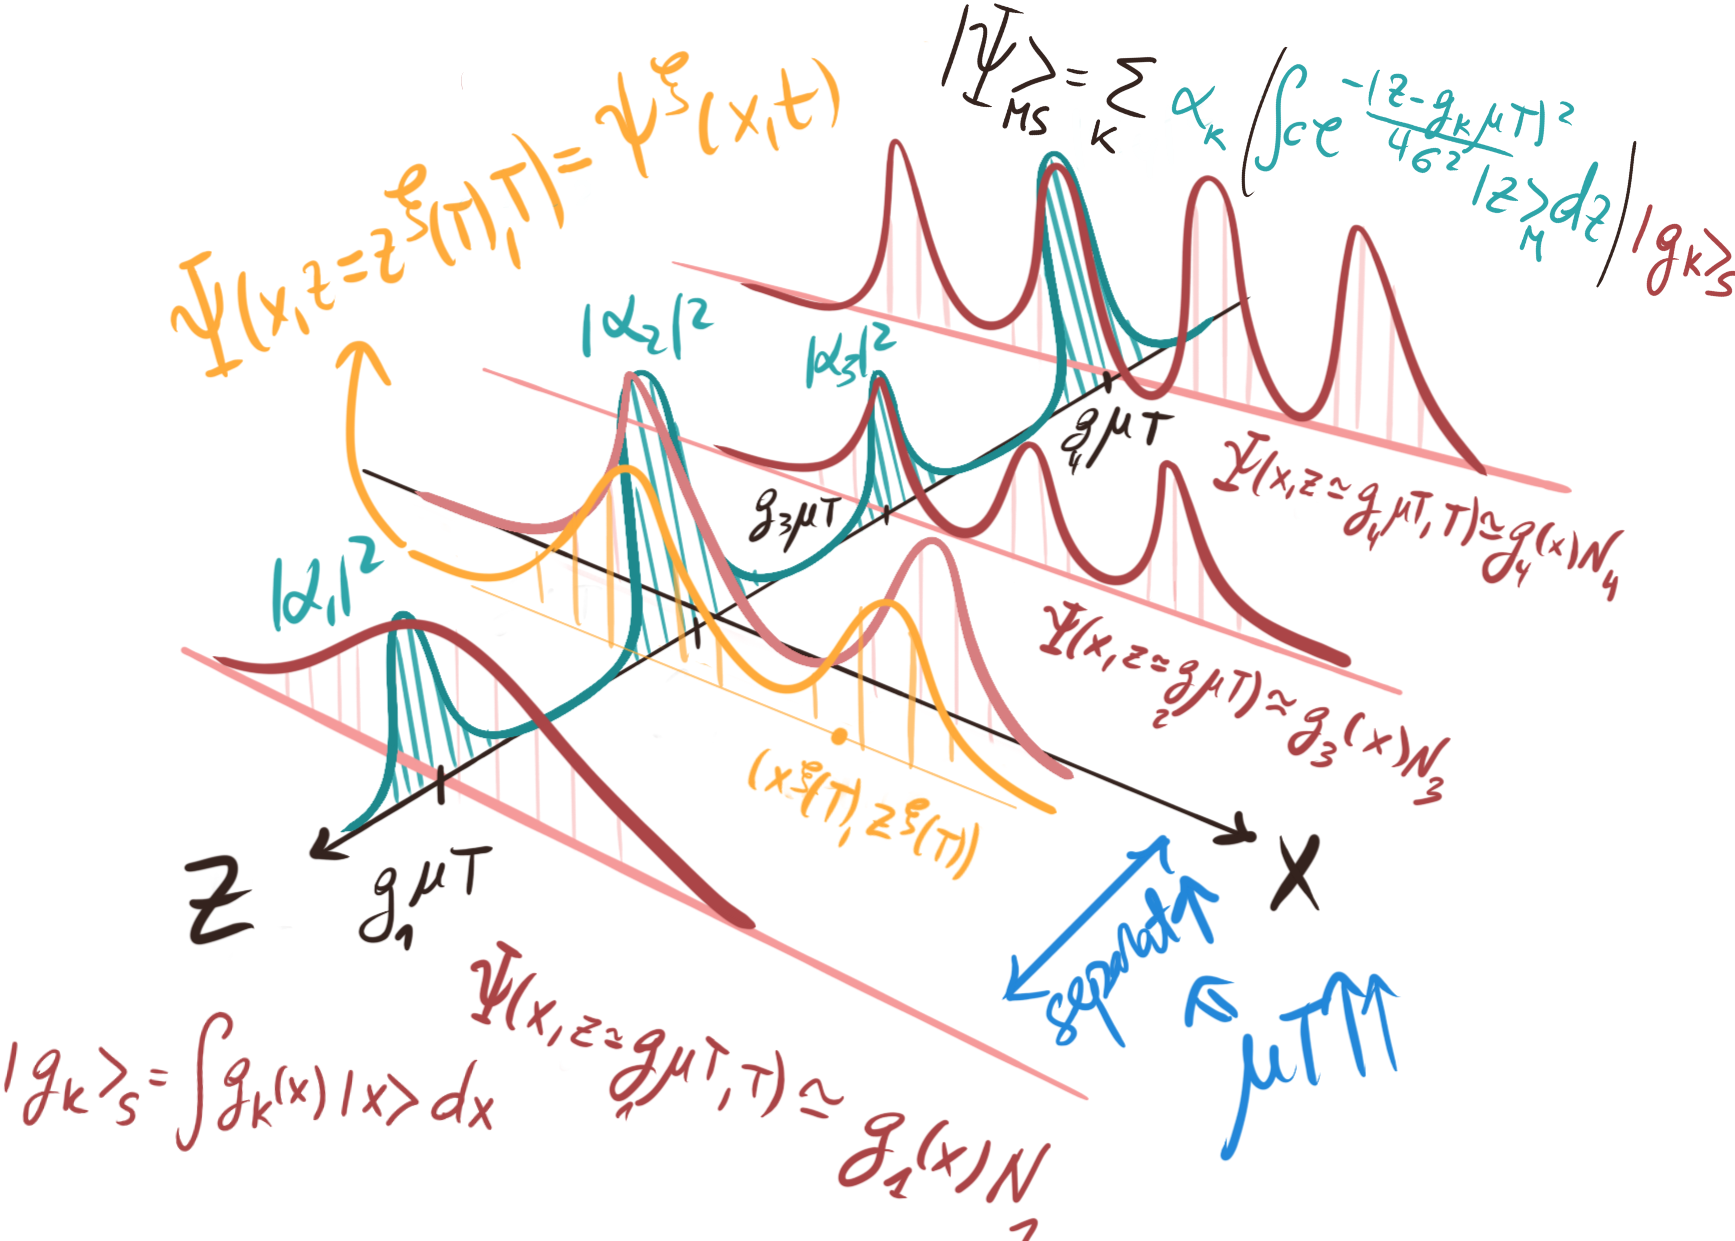
\includegraphics[width=\linewidth]{Figures/Countable.png}
    \caption{Countable Spectrum}
     \end{subfigure}
\begin{subfigure}[b]{0.45\linewidth}
    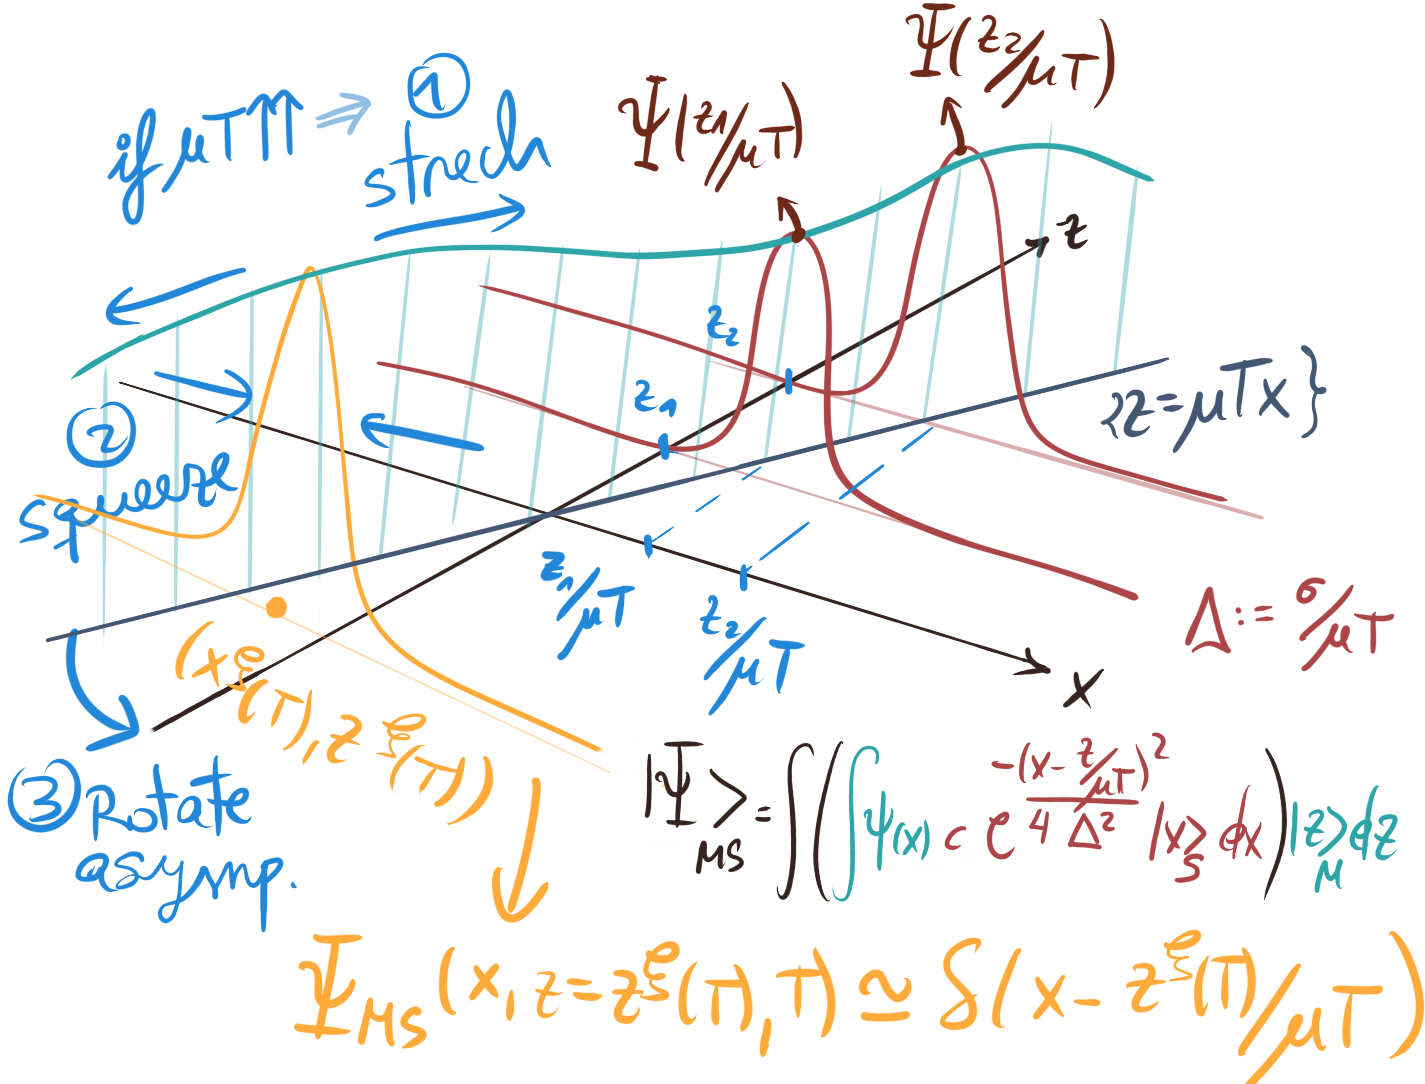
\includegraphics[width=\linewidth]{Figures/Uncountable.png}
    \caption{Uncountable Spectrum}
     \end{subfigure}
   \caption{Representation of the effective collapse of a 1D ($n=1$) system, as explained in the text. In yellow the CWF of the system, which will be the EWF when normalized. $N_k$ represents the norm of the CWF. In (a), a general countable spectrum observable $\hat{G}$ is measured, in (b) the particular uncountable spectrum position operator $\hat{x}$ is measured. }
  \label{fig:collapse}
\end{figure}
% Delta sigma zati mu T jarri
% Gausianien normalizaziño konstantie
% Ezta alpha karratu en el Psi!!!
% Txikixauek ekuaziñoak eta alboz jarri putse?
% Komprobeu benetan hau emon biher dabiela eta konstante de normalizaziñoa
% Ikusi lo de la norma de la  CWF!
% Putse leyendan jarri zer dan g(x). Ta jarri ke en el uncountable spectrum dibujas la variable positición, pero ke si se representa otra, g orduen tal!


\newpage
In both cases, as seen from the S alone, it will have looked like the unitarily evolved state $\ket{\psi}_S$ "collapsed" into one of the eigenstates of $\hat{G}_S$, with a probability equal to the pre-measurement state's projection magnitude squared $|\alpha_k(0)|^2$ (or pdf $|\psi(g,0)|^2$). This EWF will now continue to be unitarily and independently evolvable (for it will be an EWF with no interaction with M). The randomness of the measurement thus, arises due to the fact that we cannot know $z^\xi(0)$ with an arbitrary precision, unless we made a projective measurement on it before the experiment. But such a measurement as seen, would require the coupling with another ancilla indicator and so on, until the chemicals in the perception of the observer, which is known as the von Neumann chain of observation \cite{vonNeumann}.\footnote{In reality, we cannot really couple the apparatus dial M directly to the S, nor we as observers with organic detectors are directly coupled to the dial M. Yet, we can couple the S to an order of magnitude bigger ancilla $A_1$, which will be coupled to a bigger ancilla $A_2$, and so on until $M$, and then until our perceptual observation, which due to the determinate Bohmian trajectory of its constituents, lets us know the result of the measurement. This discussion is in fact a restatement of the absolute uncertainty \cite{Absolute}.} The point is that a proper description of this chain (like the Bohmian one), allows us to decide where arbitrarily between the observer and the S we place the effective "collapse", which was a requirement placed by von Neumann himself \cite{vonNeumann, NeumannNoCollapse} over his axiomatization even if it is mainly ignored by the Orthodox\footnote{He did not believe in a physical collapse \cite{NeumannNoCollapse}, instead he believed an explanation of the measurement should be possible setting an apparent collapse at an arbitrary point of the measurement Neumann chain, which is what we allow with the Bohmian description.}.

Now, either the assumption that for time $t>T$, M does not interact anymore with the S, or that the environment entanglement with the S is lost by some sort of thermalisation, mean that the information of the subsystem that was "leaked" to the environment (the so called "empty waves", which are the rest of CWF-s that are not sliced at $z=z^\xi(T)$), do not interact back\footnote{ They technically could if say, their macroscopic separation was made microscopic again. } with the EWF of the S. Any of these two assumptions thus imply that the environment effectively forgets the entanglement achieved with the S. This is an environment behavior we could call memory-less or Markovian.

Since the description of the E will only be useful for the measurement time interval $(0,T)$, and we can then discard it (as we consider it for an ideal measurement to be Markovian), we can instead explain the projection of the state of the S to a subspace of its Hilbert space, with a set of effective-"collapse" orthogonal projectors $\{\hat{\Pi}_k\}_k$ without the need to explicitly formalize M \cite{Durr}. We shall not forget however that this is just a short-cut in the modeling.

If we were now interested on the post-measurement description of the S, but irrespective of the measured result, we could independently unitarily evolve each of the different possible projected states (EWF-s), rememebering which was the probability for each of them. Then if a second measurement is performed at a later point, we could simply treat a measurement on each of the independent states and weight them with the joint probability of the previous and the current measurements. For the sake of compactness, we could instead build a "matrix" operating on states where we set the orthogonal EWF-s as the ket-bra-s with their probabilities as coefficients. If we now apply a linear operator and its Hermitian conjugate at each side of the matrix (say, a unitary evolution), we will be applying the operator to each state-vector independently of the rest. Just as we wanted. Thus, we define an operator on state-vectors, to be used as a "possible state-probability pair" container:
\begin{equation}\label{dens}
\hat{\rho}_S(T) =\sum_k |\alpha_k(0)|^2\ket{g_k}_S\bra{g_k}_S \quad \text{or} \quad \hat{\rho}_S(T)=\int |\psi(g,0)|^2\ket{g}_S\bra{g}_S dg
\end{equation}
This is the so called {\bf density matrix} of the S \cite{vonNeumann, Durr, Holland}. Note that for subsequent unconditional measurements, measurements in which we wish to keep track of all possible outcomes, the density matrix will get more and more mixed (the squared trace will diminish).\footnote{Note that these are "diagonal" representations of the density matrix but we could equivalently express them in other bases, which means we can loose the microscopic deterministic detail of what is happening if the density matrix is all that is specified. Yet, for a probabilistic operational description of S (an epistemological description), this will suffice as we will see. Yet, if the Universe is to be taken as a pure state, a density matrix can always be seen as representing human uncertainty \cite{Generalized}.} We say it is pure when we can represent it as a container describing a state with probability 1. 

\subsubsection*{A Bohmian Narrative for General Quantum Operations}
At this point, notice that the effective-"collape" due to a macroscopic separation in configuration space for different CWF-s, is not necessary to be part of a measurement by an observer. It could also happen as the effect of a more general environment coupling. 
%From the perspective of the S, such an interaction with the environment could be seen as a non-unitary evolution that makes the density matrix of the system get more mixed. Yet, a requirement for this environment, that acts as an ideal projective measurement, is that the portion of the enviornment that got entangled with the subsystem and caused its effective collapse rapidly thermalizes or never again interacts with the subsystem. This is a possible narrative for a general Markovian environment.
For example, if part of the environment gets entangled with S and this environment is projectively measured, the S will also seem to suffer an effective-"collapse", but now into non-necessarily orthogonal nor linearly-independent states (nor a number of states limited by the dimensionality of its Hilbert space). 

This example is in fact what is called a {\bf generalized measurement} \cite{Generalized, Durr}. Given a decomposition of an initial state $\ket{\psi}_S$ in a sum of not necessarily linearly-independent states of S and an independent fiducial state $\ket{\theta}_A$ for an ancilla A, by using a suitable unitary $\hat{U}_{AS}$, we could couple each state of the decomposition of $\ket{\theta}_A$ with a different state of an orthonormal basis $\{\ket{m}_A\}_m$ of A: $\hat{U}_{AS}\ket{\theta}_A\otimes\ket{\psi}_S=\sum_m \ket{m}_A\otimes \ket{\psi_m}_S$ where $\ket{\psi_m}_S:=\bra{m}_A\otimes\hat{Id}_S \qty(\hat{U}_{AS}\ket{\theta}_A\otimes\ket{\psi}_S)$ is an unnormalized S state called the {\bf conditional state} of S for the $m$-th observation of the environment A. If we now perform an ideal projective measurement on A for the $\{\ket{m}_A\}_A$ basis (coupling a dial M to A and branching A in EWF-s consisting of the measured eigenstates), ancilla-subsystem (unnormalized) EFW-s $\ket{m}_A\otimes \ket{\psi_m}_S$ would be generated as a function of the Bohmian position of the dial. The $m$-th result would be observed with a probability equal to the norm of its conditional state $N^2:=|\bra{\psi_m}\ket{\psi_m}|^2$. If we then set-off the interaction between A and S for all future times, the S will have seemed to "collapse" into the EWF $\ket{\psi_m}_S/N$ with probability $N^2$, since it will now evolve independently of $A$.

As with the projective measurement of S, we can shortcut the formalization of the A and its measurement, by just considering the general measurement operators on the S (called POVM-s) $\{\Omega_m:=\ket{m}\otimes\hat{Id}\hat{U}_{AS}\ket{\theta}_A\otimes\}_m$. The only requirement for them is: $\sum_m \Omega_m^\dagger\Omega_m=\hat{Id}_S$, so that the $m$-probabilities add-up to one, which is satisfied because $\Omega_m\ket{\psi}_S=\ket{\psi_m}_S$ is the (unnormalized) conditional state, the squared norm of which is the probability to observe $m$ \cite{Generalized, Durr}. The reason why such an A and $\hat{U}_{AS}$  exist for any set of linear operators $\{\Omega_m\}_m$ satisfying the stated restriction, will be seen in a moment. Note that we could describe the post-measurement S unconditionally, using the density matrix idea just the same way as with projective measurements, defining $\hat{\rho}_S=\sum_m \ket{\psi_m}_S\bra{\psi_m}_S$ (or an integral). A second measurement on S would straightforwardly further mix the matrix.

The so called partial trace operation is tigthly related to this. Given a density matrix $\hat{\rho}_{AS}$ for a composite A$\otimes$ S and an arbitrary orthonormal base of the A $\{\ket{m}_A\}_m$, the partial trace of $\hat{\rho}_{AS}$ over A is defined as: $tr_{A}[\hat{\rho}_{AS}] := \sum_k \bra{m}\otimes \hat{I}_S(\hat{\rho}_{AS})\ket{m}\otimes \hat{I}_S$ (or an integral if the "base" is made of uncountable improper states) \cite{Generalized, Durr}. We call the result, the {\bf reduced density matrix} of S. It can be easily proven that the partial trace yields the same result irrespective of the employed basis of A.

Its relation with measurements is the following one. The partial trace of M on the pure state $\ket{\Psi(T)}_{MS}\bra{\Psi(T)}_{MS}$ of equations \eqref{postM1},\eqref{postM2}, under the effective "collapse" conditions for $g,T,\sigma$, precisely yields the unconditional post-measaurement density matrix of equation \eqref{dens}. The same happens in any generalized measurement: the partial trace of A in $U_{AS}\ket{\theta}_A\otimes\ket{\psi}$ will yield the unconditional post-measurement density matrix $\hat{\rho}_S=\sum_m \ket{\psi_m}_S\bra{\psi_m}_S$. In general, this indicates that the partial trace of an ancilla partition A of a composite Hilbert space A$\otimes$S can always be interpreted as how the S would be left if an unconditional ideal projective measurement was performed on the A \cite{Generalized}. Note very importantly that if the traced out partition is not projectively measured (coupling a measurement ancilla to it and evolving until macroscopic distinguish-ability is achieved) and the interaction between A and S is not thermalized or does not cease indeterminately, then the reduced density matrix of S will just be a "fiction", that will not evolve  independently of A, as does happen in the case of a real measurement. Each CWF of the S for different A states (which we placed in different slots of the matrix after partial tracing) will still interact with each other since they are not EWF-s. It is still true that for statistical measurement predictions about the S, the information in the reduced density matrix will be enough. Thus, under Bohmian mechanics, the reduced density matrix is in general just a "ficticious" "how the S would be left if", useful to predict single-time measurement statistics on S. %In general though, it will be "ficticious" representation of how S would be left if the rest was unconditionally projectively measured. %Unless of course, a real unconditional measurement of A is performed (by an outer environment or by an observer) and the A-S interaction ceases. Interesting enough, the observable measured on the traced out partition is irrelevant for the resulting reduced density matrix, which is what allows the versatility of the so called pure unravellings.


In order to finish integrating the density matrix formalism and any general quantum operation (including the generalized measurements) with this Bohmian view, we can invoke the Gelfand-Naimark-Segal theorem \cite{GNSTheorem, Generalized}. By this theorem, we can assure that for any most general operation we can perform on a density matrix $\hat{\rho}_S$ of a system S (any complete-positive, convex linear and not trace increasing superoperator acting on S), say, for the operation $\mathfrak{S}$, there exists at least an ancilla system A with a pure state $\ket{\theta}_A$ and a coupling unitary evolution $\hat{U}_{AS}$ such that:
\begin{equation}
\mathfrak{S}[\hat{\rho}_S]=tr_A\qty[ (\hat{\Pi}_A\otimes \hat{Id}_S)  \hat{U}_{AS}\qty(\ket{\theta}_A\bra{\theta}_A\otimes \hat{\rho}_S)\hat{U}_{AS}^\dagger]
\end{equation}
which can be interpreted as a unitary coupling of the initially independent S and A, and posterior partially selective ideal projective measurement of $A$ (where only the eigenstates of non-null eigenvalue of $\hat{\Pi}_A$ are left and the rest are discarded). In particular, if the coupling of S and A perfectly entangles the eigenstates of $\hat{\Pi}_A$ with some orthonormal basis of S, this will be a projective measurement of S. Else, it will be a generalized measurement of S. In the trivial case where $\hat{U}_{AS}=\hat{U}_A\otimes\hat{U}_S$ and $\hat{\Pi}_A=\ket{\theta}_A$, it will just be the Schrödinger unitary evolution of S.


\subsubsection*{Markovian to Non-Markovian measurement contexts}
Following the Markovianity idea we pragmatically defined earlier, we could call a Markovian open quantum system, any evolution of the reduced density of the S that could be equivalently interpreted as if a different portion of the environment (a different ancilla) instantly got coupled every $\Delta t$ with the S and was then ideally measured, in a way that this ancilla never again interacted with the system (or their entanglement was somehow "thermalized" before their next interaction). This is equivalent to a generalized measurement of S every $\Delta t$. Among others, the "Past-Future Independence" definition of Markovianity by Wiseman {\em et al.} \cite{MarkovianityDefs}, perfectly matches this view.

In fact, as shown by Ref \cite{continousMeas}, such a continuous monitorization of different ancillas that get coupled to the system at each time, can be used to derive one of the most general dynamical equations for the reduced density matrix of a subsytem in a Markovian environment, a so called Lindblad master equations \cite{Generalized, MarkovianityDefs}. Then the derivation of an arbitrary Markovian environment master equation requires the consideration of several continuous measurements for different properties of the bath \cite{continousMeas, MarkovianityDefs}.

The fact that the dynamics of the reduced density matrix of a subsystem can be understood in these terms means that instead of trying to solve the Markovian master equation, we could do the following. Find an observable $W$ for some (fictitious or not) environment ancillas, E, ancillas that get entangled with S and are then projectively measured, producing the same average (unconditional) effect on the reduced density of S as the predicted one by the master equation (which is always possible for a Markovian E sa said). Then, we could evolve a pure state-vector of the S choosing at each projective measurement of the bath, one of the possible stochastic conditional states. This would generate a linked in time S pure state $\ket{\psi_{w(t)}(t)}_S$, associated to the result of a certain continuous measurement (or unravelling) of the bath ancillas: $w(t)$\footnote{Remember that at each time a different generalized measurement is performed on S, meaning this stochastic trajectory $w(t)$ reflects the Bohmian positions of different measurement dials at each $\Delta t$ step. Thus, its non-differentiable nature is not a problem for Bohmian mechanics.}. This pure state is called a {\bf quantum trajectory}, linked to a "noise realization" $w(t)$ for its environment \cite{Generalized, MarkovianityDefs, QuantumTrajs}. As we saw previously that the reduced density matrix of a subsystem is how it would be left if an unconditional ideal measurement was performed on the rest of the system, this tells us that we should be able to recover the reduced density for the S by averaging the ensemble of all possible quantum trajectories for the unraveling of the $W$ observable of the bath ancillas \cite{MarkovianityDefs,QuantumTrajs}:
\begin{equation}
\hat{\rho}_S(t):=tr_{ES}[\hat{\rho}_{ES}(t)]=\mathbb{E}_{w(t)}\qty[\ket{\psi_{w(t)}(t)}_S\bra{\psi_{w(t)}(t)}_S]
\end{equation}

Computationally, this means that if we got an equation ruling the stochastic time evolution of a pure quantum trajectory $\ket{\psi_{w(t)}}_S$ and its noise realization $w(t)$, we would be able to compute in parallel the density matrix using simpler data structures (vectors) \cite{MarkovianityDefs, QuantumTrajs}. Additionally, the obtained reduced density matrix is necessarily positive definite by construction. Equations of these kind are the so called, {\bf Stochastic Schrödinger Equations} (SSE-s) \cite{Generalized, continousMeas}. Note that such a pure state trajectory for a Markovian E, can always be physically interpreted in the Orthodox explanation, as a so called pure unravelling \cite{MarkovianityDefs} (where one would invoke the collapse at each $\Delta t$). In the Bohmian view a quantum trajectory is exactly a normalized CWF of the S (in ket notation), which every significant $\Delta t$ is converted into an EWF (thus the normalization).

%From our Bohmian perspective, this works because at each time $t$, the ideal measurement of the environment portion A entangled with the system S, makes the A-S CWF obtained by conditioning the A-S-measurement-apparatus wavefunction to the dial position $w(t)$ be converted into an EWF, just as explained when describing the narrative for POVMs. As was clear for POVMs in general, notice again that the measured property of the bath, indicated by $w(t)$, does not need to be its position (even in Bohmian mechanics). It is the position of the dial measuring the property of the bath, that must be a position (which is actually what $w(t)$ is in each time, assuming the Bohmian postulate that a measurement is always a position measurement in the end). 

However, what if we had an E that gets entangled with S, but which never really allows us to consideran effective collapse? What if the different CWF-s of the S, were allowed to interact in any future time, and were not converted into EFW-s every $\Delta t$? That is, what if the "quantum trajectories" could interact between them, such that the evolution of each of them depended on the rest? Then "the information leaked" onto the environment from S (the "empty waves"), would be able to affect back S in any significant future time for S. Such an environment with "memory" of the entanglement achieved with S would be called a non-Markovian environment \cite{MarkovianityDefs}. Then, it turns out that from a Bohmian interpretation, we could still continue talking about "pure state quantum trajectories", which would be the CWF-s for S (in any desired representation), conditioned on a position for the environment interacting with S (or conditioned on the position of a dial coupled with an arbitrary observable of the E interacting with the S) \cite{NMisModal, interpretSSE}. Since measurement and collapse are just described as another unitary evolution of the whole, while the positions and derived properties are ontologically real at all times, then there is no interpretative issue.

Contrarily, in the Orthodox view, a CWF (normalized or not and in any representation basis), does not have a physical interpretation, unless it is an EWF, say, unless the conditioning variable is projectively measured. As a consequence, if a SSE is found for a non-Markovian dynamical equation ruling a reduced density matrix, the conditional pure state evolved by the SSE in the Orthodox view can only be understood as the state in which S would be left on, if the E was measured...but since it is non-Markovian, we cannot assume the E is being projectively measured! If it was, the evolution of the state would be pretty different (we would neglect the interaction between the CWF-s stacked along the E axes). Thus, the linking of such states in time, can only be understood if we get out of the Orthodox and use concepts like the CWF of the Bohmian view \cite{NMisModal, interpretSSE}. Of course, mathematically, one could derive such non-Markovian SSEs as pragmatical computational tools to reconstruct the reduced density matrix, but one would need to avoid any additional consideration for the quantum trajectory (like two-time correlation computations) unless one accepts some sort of ontological reality (independent of measurement) for the conditioning property of the environment.

From the Bohmian perspective it is easy to notice why SSE-s for non-Markovian environments will not be exact in general. One of the main properties a SSE needs to have is that it should allow the time evolution of a single conditional state independently of the rest of possible conditional states, which is precisely asking that there is no quantum influence between adjacent CWF-s, influence which as explained in the beginning is the main characteristic of quantum mechanics (the quantum wholeness). In fact, this is asking for these CWF-s to be EWF-s as we saw, which would then allow a Markovian interpretation for the SSE, and thus a contradiction. Yet, SSEs that approximate the dynamics for ad-hoc cases are indeed possible in non-Markovian environments \cite{ Diosi, WisemanSSE, Thz}. This is because, an ensemble of CWF-s does not need to be an ensemble of EWF-s to allow the computation of the reduced density matrix at each time!\footnote{In fact, a whole set of CWF-s, if the system state was not mixed, would also allow the reconstruction of the full wavefunction! In which case a reduced density matrix would not even be necessary.} 

To see that this is so, independently of the nature of the environment, let us prove it for an arbitrary composed pure state (the generalization to mixed states is then trivial). Given the arbitrary state $\ket{\Psi}_{ES}$ for the environment E and system S, with position observables $\vec{y}$ and $\vec{x}$ respectively, just as introduced in the beginning\footnote{Note that since Bohmian trajectories do not cross each other in configuration space, if we sampled only Bohmian trajectories for which $\vec{x}(t_0)$ is a single position, at each time, we would still have a CWF per each position in $\vec{y}$. Thus, we have that the states $\qty{\ket{\psi^{y(\xi,t)}(t)}_S:=\bra{y(\xi,t)}_A\ket{\Psi(t)}_{AS}}_{y\in\R^{N-n}}$ are all the possible slices of the $\vec{y}$ axis.}:\vspace{-0.2cm}
\begin{equation}
\ket{\Psi(t)}_{AS}=\int\ket{\vec{y}^\xi(t)}_A\otimes \ket{\psi^\xi(t)}_S d\xi = \int\ket{\vec{y}}_A\otimes \ket{\psi^{y(\xi,t)}(t)}_S dy
\end{equation}
Then tracing out A in $\hat{\rho}_{AS}(t)=\ket{\Psi(t)}_{AS}\bra{\Psi(t)}_{AS}$, we would get the reduced density for S:
\begin{equation}
tr_E\qty[\hat{\rho}_{AS}(t)] = \int\bra{\vec{y}}\hat{\rho}_{AS}(t)\ket{\vec{y}}dy = \int \ket{\psi^{y(\xi,t)}(t)}\bra{\psi^{y(\xi,t)}(t)} dy = \mathbb{E}_{y(\xi,t)}\qty[\ket{\psi^{y(\xi,t)}(t)}\bra{\psi^{y(\xi,t)}(t)}]
\end{equation}
Thus, the ensemble average of the CWF-s reproduces the reduced density.

This clear narrative in terms of Bohmian CWF-s for non-Markovian open quantum systems is not only theoretically insightful, but is a {\bf practical} tool to look for reasonable SSE-s. To exemplify this, let us describe two practical frameworks we developed.

\subsubsection*{Non-Markovian SSE for two-terminal electronic devices operating at THz frequencies}
%In the pragmatical view we have mentioned about Markovian open quantum systems, we said the dynamics should be interpretable as if every $\Delta t$ a POVM (instantaneously for S) took place. This means that in such a picture, the entanglement and interaction bewteen the subsystem and the enviornment should decay in a time scale $\tau_{decay}$ much smaller than any characteristic time scale for the subsystem $\tau_S$ (related with $\Delta t$), $\tau_S>>\tau_{decay}$. However, 
Following Bohmian mechanics and Ref.\cite{GJ}, we have already shown after equation \eqref{SE.GJ}, a way to obtain SSE-s for arbitrary settings. In principle, in those equations the CWF of the S and the E one are coupled at all times, not only between them, but also with the rest of possible CWF-s (non-Markovianity). However, for specific scenarios, we can make educated guesses for the quantum correlation terms $G$ and $J$, and the classical potential $U$, to render a SSE for individual CWF-s of the S.

For nano-scale electronic devices operating at very high frequencies (in the order of THz), both the relevant dynamics of the S and the measurement coupling times are below picoseconds time-scales, implying Markovian assumptions for encironment coupling are meaningless: there is "no time for their entanglement to be forgotten" \cite{Thz}. This problem for a two-terminal nano-electron device is approximated in the BITLLES simulator \cite{tdp,Pois,Thz}, as an application example of the mentioned method. For this, the classical potential is evaluated through the solution of the Poisson equation\cite{Pois}, while $G$ and $J$ are modeled by a proper injection model \cite{inject} as well as proper boundary conditions \cite{boundary1, boundary2} that include the correlations between the active region of the two-terminal nano-device and the reservoirs. Even electron-phonon decoherence effects can be included effectively \cite{eph}.

The number of electrons contributing to the electrical current , the observable of interest, are mainly those in the active region of such a nano-device, which we consider thus, the subsystem S of interest. This number $n/3$ fluctuates as there are electrons entering and leaving this region. Such a "creation and destruction" of electrons from the point of view of S, leads to an abrupt change in the degrees of freedom of its CWF. This problem can be circumvented in Bohmian mechanics by decomposing the CWF of S, $\psi^{y^\xi(t)}(\vec{x},t)$, into a set of CWF-s for each electron. That is, for each of the $n/3$ electrons of position $\vec{x}_k:=(x_{3k+1}, x_{3k+2}, x_{3k+3})$ with $k\in\{0,..,n/3-1\}$, we define a single particle CWF $\phi_k^\xi(\vec{x}_k, t):=\psi^{y^\xi(t)}(\vec{x}_k, \vec{x}_{\neg k}=\vec{x}_{\neg k}^\xi(t),t)$ with $\vec{x}_{\neg k}=(\vec{x}_1,..,\vec{x}_{k-1}, \vec{x}_{k+1}, ...,\vec{x}_{n/3})$. Then, we can consider a set of $n(t)/3$ equations like \eqref{SE.GJ}, one for each of the electron, to evolve each $\phi_k^\xi$. Note that what we have just done is to consider S, the subsystem of the non-Markovian open quantum system, as itself composed of several open quantum systems that will interact with each other in a non-Markovian way.

Now, the active region of the electron device S, is connected by a macroscopic cable (representing the portion of the environment A that gets entangled with the S) to an ammeter (acting as a measuring apparatus M). The electrical current read by the Bohmian position of the dial in the ammeter (correlated with the Bohmian trajectory of the charge carriers in the cable, which are correlated with the electrons in the active region) is the observable we want to predict. Thus, in principle the evaluation of the electrical current should require keeping track of all the environment degrees of freedom. However, it is known that the total current density defined as the sum of the particle and displacement currents, is a divergenceless vector \cite{diver1, diver2}, which makes the total current evaluated at the ends of the active region be equal to the total current evaluated at the cables. It is additionaly known \cite{equiv} that since the cable, unlike the active region, has macroscopic dimensions, the current at the ends of the active region is only due to the electrons in the active region (plus a nearly white noise). This is qualitatively because the electrons in the metallic cables have a very short screening time, meaning the electric field generated by an electron in the cable spatially decreases rapidly due to the presence of many other mobile charge carriers in the cable that screen it out. Thus, the contribution of these outer electrons to the displacement current at the border of the active region is negligible \cite{neg}. Therefore, the variable of the environment associated to the total current $z(t)\equiv I(t)$ can indeed be equivalently computed at the boundary of the S. Finally, such a current (its expected value), can be computed from the Bohmian trajectories of the electrons in the active region as we will later explain. 

In Ref. \cite{Thz} we provide some numerical results demonstrating the ability of the presented method, by simulating a two-terminal electron device whose active region is a graphene sheet, contacted to the outer by two (ohmic) contacts. Here, to further take into account the electromagnetic environment of the electron device, we model the interaction between the graphene device and the environment through a resistor and a capacitor in series. The details are found in the mentioned article. 

\subsubsection*{Towards another general framework to look for position SSEs}
We have developed a second framework to look for SSEs (equations to evolve CWF-s independently), based on the Born-Huang ansatz of the full wavefunction, at the cost of having a suitable guess for the conditional energy eigenstates of the relevant parts of the environment. For this, given the full, subsystem-environment Hamiltonian $\hat{H}(\vec{x},\vec{y},t)=\sum_{k=1}^N \frac{-\hbar^2}{2m_k}\pdv[2]{}{x_k} + U(\vec{x},\vec{y},t)+V(\vec{x},t)$, \footnote{The classical potentials are allowed to have a time dependence to account for classical interaction with the rest of the environment.} we can define the transversal section Hamiltonian as $\hat{H}_x(\vec{y},t):=\sum_{k=m+1}^N\frac{-\hbar^2}{2m_k}\pdv[2]{}{x_k}+U(\vec{x},\vec{y},t)$. Then, we define the set of eigenstates $\{\Phi^j_x(\vec{y},t)\}_j$ with eigenvalues $\{\varepsilon_x^j(t)\}_j$, parametrized by the chosen section $\vec{x}$, to be the solution of: $\hat{H}_x(\vec{y},t)\Phi^j_x(\vec{y},t)=\varepsilon_x^j(t)\Phi^j_x(\vec{y},t)$. We call these $\Phi^j_x(\vec{y},t)$, transversal section eigenstates (TSE). Since the hermiticity of the operator $\hat{H}_x(\vec{y},t)$ implies the TSE-s form an orthonormal basis for the Hilbert space of $\vec{y}$ at each $\vec{x}$, we could expand the ansatz: $\Psi(\vec{x},\vec{y},t)=\sum_j \Lambda^j(\vec{x},t)\Phi_x^j(\vec{y},t)=\sum_j \varphi_j(\vec{x},\vec{y},t)$, with $\Lambda^j(\vec{x},t):=\int\Phi^j_x(\vec{y},t)\Psi(\vec{x},\vec{y},t)dy$ the projection coefficients and $\varphi_j(\vec{x},\vec{y},t):=\Lambda^j(\vec{x},t)\Phi^j_x(\vec{y},t)$.

Now, using this expansion in the Schrödinger Equation, and evaluating the full wavefunction along the trajectory for the environment $\vec{y}=\vec{y}^\xi(t)$\footnote{In reality, we could choose any trajectory we like for the environment if we are not interested in computing Bohmian trajectories. Thus, it could be the result of a measurement of the environment, or just a set of trajectories that leads us to the construction of the reduced density with the least number of them.}, we can get by denoting $\varphi^k_\xi(\vec{x},t):=\varphi^k(\vec{x},\vec{y}^\xi(t),t)$ that:
\begin{equation}
 i\hbar\pdv{}{t}\varphi^k_\xi(\vec{x},t)=\qty[-\sum_{s=1}^m\frac{\hbar^2}{2m_s}\pdv[2]{}{x_s}+ \varepsilon^k(\vec{x},t)+V(\vec{x},t)   +i\hbar \dv{}{t}log(\Phi^k_x(\vec{y}^{\, \xi}(t),t))]\varphi^k_\xi(\vec{x},t)+
\end{equation}
$$
\hspace{-0.4cm}+\sum_{j=0}^\infty\sum_{s=1}^m \frac{-\hbar}{2m_s}\qty( \frac{1}{\Phi^j_x(\vec{y}^{\, \xi}(t),t)}\pdv[2]{\Phi^j_x(\vec{y}^{\, \xi}(t),t)}{x_s}+2\pdv{}{x_s}log(\Phi^j_x(\vec{y}^{\, \xi}(t),t))\qty[\pdv{}{x_s}-\pdv{}{x_s}log(\Phi^j_x(\vec{y}^{\, \xi}(t),t))] )\varphi^j_\xi(\vec{x},t)
$$

Because the CWF for the subsystem can be recovered from $\psi^\xi(\vec{x},t)=\sum_j \varphi^j_\xi(\vec{x},t)$, we have obtained a set of exact linear equations involving only $n$ dimensional states (instead of $N$) that allow the evolution of single CWF-s. In principle, since a general Hilbert space will need to have a countably infinite number of orthonormal states in a basis, it would be a set of infinite number of equations. However, we shall reasonably truncate the expansion of the CWF at a relatively low fixed point (at which for example the norm of the CWF surpasses a certain threshold), or even allow it to vary in time. If so, the difficulty of these equations would only relay on the knowledge of the TSE-s $\Phi^j_x(\vec{y},t)$. The point is that providing educated guesses for them seems to be more reasonable than guessing for $G$ and $J$, and might be a starting point for the derivation of ad hoc SSE-s for particular non-Markovian environments.  \vspace{-0.2cm}

 
\subsubsection*{Properties of the Pilot Wave or Properties of the Trajectory? \\ Can we predict all observables using Bohmian trajectories?}

From the provided narrative, we can see that a measurement operator $\hat{G}=\sum_g g\ket{g}\bra{g}$, is just a way to gather an orthonormal basis $\{\ket{g}\}_g$, where each $\ket{g}$ is linked with a value $g$. We also saw that a projective measurement that uses $\hat{G}$ in its interaction Hamiltonian, reveals the {\bf post}-measurement state $\ket{g}$, as a function of the measured $g$, which will happen with a probability due to the {\bf pre}-measurement state. With enough repetitions, we could end up knowing these probabilities, which are related to the projection of the the pre-measurement state onto the possible post-measurement states. Beyond serving to reveal the post-measurement state and pre-measurement state's projection coefficients, in the provided Bohmian view, the measured value $g$ related to $\hat{G}$, is devoid of any additional meaning (unless $\hat{G}$ is a function of the position operator, in which case we say what we measured is the post-measurement property of a Bohmian trajectory). But then, in general, is this $g$ (say for a momentum, an energy or a spin measurement) just a mathematical tool? That is, we cannot say $g$ is a property of the wavefunction, since otherwise we would need to say that a state in superposition has multiple simultaneous observable values. But apparently, we cannot either say it is a property of the Bohmian trajectory. But then, if "measuring" as Bell said \cite{Bell}, is about revealing information of the unmeasured (pre-measurement) system: are the projection probabilities the only thing we can really know about the unmeasured system? This debate was not experimentally interesting until recently the community acknowledged that some properties predicted for Bohmian trajectories could indeed be experimentally measured, when Wiseman proposed his protocol to operationally measure the Bohmian velocity of a pre-measurement system \cite{WisemanVel}.

More recently, some of the authors derived a very insightful observation that extends this concept, allowing, if wished, not only to derive an Orthodox observable operator for any property of a Bohmian trajectory, but to consider that any Orthodox observable operator (even the ones not commuting with the position operator), can always be understood as an observable property of the Bohmian trajectory, meaning this $g$ can indeed be always understood as a defined property of a trajectory \cite{DevInPosition1, DevInPosition2}. Not only that, but it was proven that, no matter if we consider this identification a simple mathematical tool, this leads to several {\bf practical} advantages in the characterization of a quantum system in the absence of observation.

Given any arbitrary (Hermitian) operator $\hat{G}$, describing the observable property $G$ for the subsystem S, with normalized EWF $\ket{\psi(t)}$, let us define the function $G^{\psi}(x,t):=\frac{\bra{\vec{x}}\hat{G}\ket{\psi(t)}}{\bra{\vec{x}}\ket{\psi(t)}}$ (which as will be discussed later on, is the weak value \cite{Weak} of $\hat{G}$ for the state $\ket{\psi(t)}$ at time $t$, post-selected at $\vec{x}$). Then, we could define a real function $G_B^\psi(\vec{x},t)=\mathbb{R}e\{G^{\psi}(x,t)\}$, which we say is the property $G$ of the Bohmian trajectory passing from $\vec{x}$ at time $t$. Until here it seems just a cumbersome definition. Yet, let us compute the expected value for $\hat{G}$ and try to write it as a function of $G^\psi(x,t)$:
\begin{equation}
\langle \hat{G}\rangle(t)= \bra{\psi(t)}\hat{G}\ket{\psi(t)}=\int \bra{\psi(t)} \ket{\vec{x}}\bra{\vec{x}}\hat{G}\ket{\psi(t)}dx =  \int |\psi(\vec{x},t)|^2G^\psi(\vec{x},t)dx
\end{equation}
which means that the spatial average of the (possibly complex) $G^\psi(x,t)$, gives the same expected value for the observable as using the operator. But here comes the most interesting point: since $\hat{G}$ is an observable, its expected value will be a real number, meaning that $\langle \hat{G}\rangle=\mathbb{R}e\{\langle \hat{G}\rangle\}$, which means:
\begin{equation}
\langle \hat{G}\rangle(t)=\int |\psi(\vec{x},t)|^2G_B^\psi(\vec{x},t)dx= \lim_{|\Sigma|\rightarrow \infty}\frac{1}{|\Sigma|} \sum_{\xi\in\Sigma} G_B^\psi(\vec{x}^\xi(t),t)
\end{equation}
where we used the quantum equilibrium hypothesis \cite{Absolute} for the set of trajectories $\{\vec{x}^\xi(t)\}_{\xi\in\Sigma}$ sampled in independent repetitions of the experiment. This equation means that the real property $G_B^\psi(\vec{x}(\vec{\xi},t),t)$ of the $\vec{\xi}$-th Bohmian trajectory, averaged over the ensemble of possible trajectories, gives the same value as the operator's expected value. This already tells us the property $G^\psi_B$ should be something. Yet, the true hit comes with the following: what would the suggested Bohmian property related with $G$ be if $\ket{g}$, an eigenstate of $\hat{G}$ with eigenvalue $g$, was the system state?
\begin{equation}
G_B^\psi(x)=\mathbb{R}e\qty{ \frac{\bra{\vec{x}}\hat{G}\ket{g}}{\bra{\vec{x}}\ket{g}} } = \mathbb{R}e\qty{ \frac{\bra{\vec{x}}\ket{\psi}g}{\bra{\vec{x}}\ket{\psi}} }=g
\end{equation}
This suggests $\ket{g}$ is an eigenstate of $\hat{G}$ if and only if it is a state for which every Bohmian trajectory has the same value of the property $G$. The implications of this are twofold. First, this says that effectively, the measured $g$ in a projective measurement, is indeed a property of the Bohmian trajectory (if we wish). Second, this is then a tool to construct the operator $\hat{G}$ itself, by defining $\hat{G}$ in terms of $G^\psi_B$ and not the other way around. We can equivalently define $\hat{G}$ as the collection of states in which all Bohmian trajectories have the same value $g$ for $G_B^\psi$. This is useful for there are observables, like the many electron current in a nano-device, for which there is no clear measurement operator, yet there is a clear Bohmian observable associated with it \cite{Pel, equiv}, as we will see.

As the icing of the cake, it turns out, as we proved in \cite{DevInPosition1}, that if we set as $\hat{G}$, the momentum operator $\hat{p_k}$ of the $k$-th degree of freedom, the Bohmian trajectory property $G^\psi_B(\vec{x},t)$ is exactly equal to the Bohmian momentum of the trajectory crossing $\vec{x}$: $m_k v_k(\vec{x},t)$. If we set as $\hat{G}$, the Hamiltonian operator $\hat{H}$, the property $G^\psi_B(\vec{x},t)$ turns out to be exactly equal to the Bohmian energy (kinetic plus classical and quantum potentials \cite{JordiXavier}) of the trajectory crossing $\vec{x}$. And the list of these "fortunate" matches goes on. Even beyond. For instance, if wished, we could have at all times a simultaneous deterministic value for the three components of spin \cite{spin}.

In summary, since we placed no restriction on $\hat{G}$, this means that for {\bf every} observable of a quantum system, we are mathematically safe (if wished), to assume that at all times, each Bohmian trajectory has an ontologically determined value for all of them. Moreover, these values will in fact evolve continuously in time, as long as wavefunctions always evolve so. This has another striking consequence: if $g$ is the observed value for a trajectory after a von Neumann coupling (thus the value we measure strongly), and the trajectory had another value for $G$ before the interaction started, then the property $G$ took all intermediate values before taking $g$, not necessarily among the eigenvalues of $\hat{G}$. Thus, if we want, we are safe to see the "quantization" of quantum mechanics as an apparent property, due to the fact that for a "proper" measurement, we require that a dial saying $g$ is compatible with a wavefunction $\ket{g}$ that will give a measurement $g$ with probability 1. That is, a wavefunction which has all its Bohmian trajectories with value $g$ for $G$. Then, we simply call it quantum because this delicate orchestration can only happen for a certain "quantized number" of states.

As if all this was not already hard to digest, there is even an additional point to be remarked. If we could really only measure $G_B^\psi$ when we forced it by a von Neumann interaction to be an eigenvalue of $\hat{G}$, all this would have no practical application. However, it turns out, we can actually measure the "unmeasured" $G_B^\psi$ for {\bf any} Bohmian trajectory. How? Well, we defined it as the real part of a weak value, a particular one we have named the "local-in-position weak value" \cite{DevInPosition1, DevInPosition2}. And as it is so well known \cite{Weak}, the real part of a weak value can indeed be experimentally measured. For this, first couple an ancilla with the subsystem of EWF $\ket{\psi}$, through the von Neumann Hamiltonian, which if coupled with a big enough interaction strength $\mu$, remember that produces the separation in macroscopically separated eigenstates of $\hat{G}$. Yet, let the interaction strength be very small, such that the system state is only slightly perturbed (just a little amount of information is leaked to the environment). Now strongly measure the slightly entangled ancilla's position (through a strong coupling of a second ancilla with the first one, then macroscopic separation etc.). This will yield a weak measurement about the S. Note the von Neumann Hamiltonian is such that no matter the strength $\mu$, the position of the ancilla will always have the same expected value as the coupled observable (in our case $G$). There is still a step more though. Right after the weak measurement of $G$ has been performed, a third ancilla is rapidly coupled to the (only slightly perturbed) S, with a coupling Hamiltonian to projectively measure the position of the S with a certain precision (according to the Bohmian view reviewed in the beginning, this position is in fact the Bohmian position of the system). Finally, we could average the weak measurements that after-wards lead us to measure the system position  at a certain $\vec{x}$. The result would be exactly $G^\psi_B(\vec{x},t)$ \cite{Weak, DevInPosition1}. One could legitimately say, this is just juggling with numbers due to several observations. But, one could also perfectly legitimately say (especially after what we have revealed) that the average weak measurements of $G$, for experiments in which the system was at $\vec{x}$, gave $G^\psi_B(\vec{x},t)$, because all the times that our Bohmian trajectory was at $\vec{x}$, the system had indeed the property $G^\psi_B(\vec{x})$. Phenomenologically this interpretation is ofcourse unprovable, yet, in the operational sense mentioned by Ref. \cite{WisemanVel}, it seems a more simple view for a pragmatic experimentalist.

\subsubsection*{Practical Applications of Local-In-Position Weak Values}


This Bohmian discovery, as already anticipated, has several practical applications \cite{DevInPosition1, DevInPosition2}. On the one hand, we can numerically predict the expected value for an observable without the need to have explicitly defined its formal operator. One can derive the observable $G^\psi_B(x,t)$ in the language of Bohmian mechanics, which is very akin to classical mechanics, and compute the ensemble average of the property to get the expected value of the operator realted to it. For example, this is how we can predict the total electrical current crossing the active region of a two-terminal nano-device operating at high frequencies (THz) \cite{equiv, Pel}. The total current at such frequencies needs to consider the displacement component (time-derivative of the electric field), which makes it hard to even ask what the current operator $\hat{I}$ should look like. However, we can define the current due to the Bohmian trajectory of a $k$-th electron $\vec{x}_k^\xi(t)$ of charge $q$ through a surface $\sigma$ as: $I_k^\xi(t)=\int_\sigma \vec{J}^\xi(\vec{r},t)\cdot d\vec{s}+\int_\sigma \varepsilon(\vec{r},t)\pdv{\vec{E}^\xi(\vec{r},t)}{t}\cdot d\vec{s}$, where $\varepsilon(\vec{r},t)$ is the electric permittivity , $\vec{J}^\xi(\vec{r},t)=q\dv{\vec{x}_k^\xi(t)}{t}\delta(\vec{r}-\vec{x}_k^\xi(t))$ the particle current density, and $\vec{E}^\xi(\vec{r},t)$ is the electric field generated by the electron, as a solution to the Gauss equation.\footnote{The legitimacy of a well defined electric field in Bohmian mechanics will be described in the last part of the chapter.} Then, as proven in \cite{Pel}, for two terminal devices of longitudinal length $L$ with metallic contact surfaces $\sigma$ of width and height $w,h>>L$, the total current contribution in the surfaces is: $I^\xi_k(t)=\frac{q}{L}v_x^\xi(\vec{x}=\vec{x}_k(t), t) $ where $v_x$ is the longitudinal direction Bohmian velocity of the electron. The total Bohmian current at the surface $\sigma$ will be the sum of these contributions $I^\xi(t)=\sum_k I^\xi_k(t)$, such that $\mathbb{E}_\xi [I^\xi(t)]=\langle \hat{I}\rangle(t)$. 
%Then by the conservation of the total current, the expectation of the current measured in the ammeter will match with the expected current in the ammeter.

As a second and perhaps the most sounded application led by this discovery: it provides an operational answer to the search of non-contextuality in the definitions of measurements involving two different times \cite{DevInPosition1}. Saying that a property of a system is contextual means that its value depends on the environment employed to convey that information to the observer. Several considerations arise here:

{\bf (1.)} We can measure a single-time (static) expectation of a property $G$ for the S, $\langle \hat{G}\rangle$, averaging the results of several quantum measurements. Which-ever fiducial state we employ in an either strong or weak measurement, the result will be the same and equal to the expectation calculable by only knowing the pre-measurement EWF of the S (thus it is a measurable non-contextual property of the S). However, it will not be as easy if we want to know the expectation of the product of two observables (time correlation), between an observable $F$ at time $t_1$ and any observable $G$ at time $t_2$. Especially if we need this information to contain exclusively information about the S (to be non-contextual). We could correlate the result of a strong measurement of $F$ at time $t_1$ and a strong measurement of $G$ at time $t_2$, but since the measurement at $t_1$ will project the state to different EWF-s, the backaction of the measuring device will be obvious. In fact, even numerically it seems hard to be well defined. If their operators do not commute, $\langle \hat{G}(t_2)\hat{F}(t_1)\rangle$ in the Heisenberg formalism will give a complex number in general. Alterantively, we could look for $\mathbb{R}e \qty{\langle \hat{G}(t_2)\hat{F}(t_1)\rangle}$ which would now be real and turns out to be the correlation of a weak measurement of $F$ at time $t_1$ and a strong measurement of $G$ at time $t_2$ (thu, also experimentally measurable). This seems to provide a "backaction-free" correlation definition for the dynamic variables. Yet, as shown in \cite{spin}, even an ideally weak measurement does in fact perturb the system in a way that is dependent, for example, on the particular fiducial state employed for it.

{\bf (2.)} Since work is a dynamical property implying at least two times, this contextuality issue has led in quantum thermodynamics a "no-go" theorem \cite{nogo} stating that there cannot exist a work superoperator that simultaneously satisfies all the physical properties required from it. Other history dependent thermodynamic properties suffer from the same issue \cite{workPb1, workPb2}: a definition of them always seems to be dependent on a particular measuring scheme, which causes as many quantum work definitions as say, acceptable measurement fiducial states exist.

{\bf (3.)} A similar issue raises when trying to measure the maximum working frequency of state-of-the-art transistors to test the performance of modern computers \cite{modern}. For this, the time spent by electrons in the active region of such nano-scale transistors, their "dwell time", must be measured. One could place position detectors in the two ends of the active region, but this metric would be unsuitable since in operation, no computer has such detectors at the ends of its transistors \cite{tunnel1, tunnel2}.

All these call for a way to paradoxically measure "unmeasured" dynamical properties of a quantum subsystem. Dynamical properties that could be predicted in a simulation without any explicit introduction of a particular measuring ancilla, but which could also be measured. As it turns out, this is exactly what the Bohmian property $G^\psi_N(\vec{x},t)$ is.

{\bf (1.)} As such, the problem of non-contextual two-time correlations of dynamical variables for a wavefunction $\ket{\psi(t)}$, can be circumvented by computing the expectation as would be done by a frequentist definition in a classical system. Given a big enough set of trajectories $\{\vec{x}^\xi(t)\}_{\xi\in \Sigma}$ each with associated ontologically deterministic observables $G_B^\psi(\vec{x},t)$ and $F_B^\psi(\vec{x},t)$, following quantum equilibrium \cite{Absolute} we could define:
\begin{equation}
\langle G(t_2)F(t_1)\rangle = \lim_{|\Sigma|\rightarrow \infty}\frac{1}{|\Sigma|} \sum_{\xi\in\Sigma} G_B^\psi(\vec{x}^\xi(t_2),t_2)F_B^\psi(\vec{x}^\xi(t_1),t_1) =
\end{equation}
$$
=  \int |\psi(\vec{\xi},0)|^2\ \mathbb{R}e\qty[ \frac{\bra{\vec{x}^\xi(t_2)}\hat{G}\ket{\psi(t_2)}}{\bra{\vec{x}^\xi(t_2)}\ket{\psi(t_2)}} ] \mathbb{R}e\qty[ \frac{\bra{\vec{x}^\xi(t_1)}\hat{G}\ket{\psi(t_1)}}{\bra{\vec{x}^\xi(t_1)}\ket{\psi(t_1)}} ]d\xi
$$
%This correlation value not only is context-free, which means is an "unmeasured" property that gives information about the system alone, but it can also be experimentally computed employing (quite a lot of) weak measurements.
{\bf (2.) } In a similar way, we can solve the problems concerning a quantum work definition as done by \cite{work1, work2}. First note that given a general system Hamiltonian $\hat{H}=\sum_k \frac{-\hbar^2}{2m_k}\pdv[2]{}{x_k}+V(\vec{x},t)$:
\begin{equation}
E^\psi_B(\vec{x}^\xi(t),t) = \mathbb{R}e\qty[ \frac{\bra{\vec{x}^\xi(t)}\hat{H}\ket{\psi(t)}}{\bra{\vec{x}^\xi(t)}\ket{\psi(t)}} ] = \sum_{k=1}^n\frac{1}{2}m_kv_k(\vec{x}^\xi(t),t)^2+V(\vec{x}^\xi(t),t)+Q(\vec{x}^\xi(t),t)
\end{equation}
with $Q$ the well known Bohmian quantum potential \cite{Holland, Durr, JordiXavier}. This proves $E^\psi_B(\vec{x}^\xi(t),t)$ is, as anticipated, the total Bohmian energy of the trajectory at time $t$. Then, following classical mechanics, we can compute its associated Bohmian work as the energy difference (if conservative, else employing an integral): $W^\xi(t_1,t_2)= E^\psi_B(\vec{x}^\xi(t_2),t_2)-E^\psi_B(\vec{x}^\xi(t_1),t_1)$. Therefore, the definition of the non-contextual quantum work would be the ensemble average of the trajectory works:
\begin{equation}
\langle W(t_1,t_2)\rangle = \lim_{|\Sigma|\rightarrow \infty}\frac{1}{|\Sigma|} \sum_{\xi\in\Sigma} \qty(E^\psi_B(\vec{x}^\xi(t_2),t_2)-E^\psi_B(\vec{x}^\xi(t_1),t_1))
\end{equation}
{\bf (3.) }Finally, we could give a reasonable Bohmian answer to the search of an "unmeasured" dwell time, as the expected time spent by the S Bohmian trajectory of the electron within the active region $\Gamma\subset \R^3$. Mathematically, the dwell time $\tau$ for the $\xi$-th trajectory of the $k$-th electron with EWF $\psi^\xi(\vec{x}_k,t)$ is by definition given by the Lebesgue integral: $\tau^\xi_B= \int_{0}^\infty  dt \int_\Gamma \delta(\vec{r}-\vec{x}_k^\xi(t)) dr$. This makes the expected time $\langle \tau\rangle$ be, by the quantum equilibrium hypothesis:
\begin{equation}
\langle \tau \rangle = \lim_{|\Sigma|\rightarrow \infty}\frac{1}{|\Sigma|} \sum_{\xi\in\Sigma} \tau_B^\xi = \int_{0}^\infty dt \int_\Gamma |\psi^\xi(\vec{r},t)|^2dr
\end{equation}
which turns out, is a well-known equation used to predict the dwell time.

%\subsubsection*{Can we understand light matter interaction through well defined "Bohmian-electromagnetic fields"?}




\newpage
\begin{thebibliography}{1}
{\footnotesize 

\bibitem{where}
Oriols X. and Ferry D. K., {\em "Why engineers are right to avoid the quantum reality offered by the orthodox theory? [point of view],"} Proceedings of the IEEE, vol. 109, no. 6, pp. 955-961, 2021.

\bibitem{Bohm}
Bohm, D. {\em "A suggested interpretation of the quanta theory in term of hidden variables: Part I."} Phys. Rev. 85, 166–179 (1952).

\bibitem{Holland}
P. R. Holland, {\em "The Quantum Theory of Motion: An account of the de Broglie-Bohm Causal Interpretation of Quantum
mechanics,"} Cambridge University Press, Cambridge 1993.

\bibitem{Durr}
Dürr D., Teufel. S. {\em "Bohmian mechanics: the physics and mathematics of quantum theory,"} Springer Science \& Business Media, Berlin, Germany, 2009.

\bibitem{JordiXavier}
	Oriols X., Mompart J., {\em "Applied Bohmian Mechanics: From Nanoscale Systems to Cosmology,"} Pan Stanford, Singapore, 2012.
	
\bibitem{Thz}
Pandey, D., Colomés, E., Albareda, G. \& Oriols, X. {\em "Stochastic Schrödinger equations and conditional states: A general non-Markovian quantum electron transport simulator for THz electronics."} Entropy 21(12), 1148 (2019).

\bibitem{Absolute}
Dürr, D., Goldstein, S. \& Zanghí, N. {\em "Quantum equilibrium and the origin of absolute uncertainty."} J Stat Phys 67, 843–907 (1992).

\bibitem{GJ}
Oriols X. {\em Quantum-trajectory approach to time-dependent transport in mesoscopic systems with electron-electron interactions} Phys. Rev. Lett. 98 066803 (2007).

%\bibitem{XOPhysSpace}
%Norsen, T., Marian, D. \& Oriols, X. {\em Can the wave function in configuration space be replaced by single-particle wave functions in physical space?.} Synthese 192, 3125–3151 (2015).

\bibitem{vonNeumann}
von Neumann, J. {\em "Mathematische Grundlagen der Quantenmechanik."} Springer Verlag, Berlin (1932).

\bibitem{NeumannNoCollapse}
Becker, Lon. {\em “That von Neumann Did Not Believe in a Physical Collapse.”} The British Journal for the Philosophy of Science 55, no. 1 (2004): 121–35.

%\bibitem{XOCM}
%Oriols, X., \& Benseny, A. {\em "Conditions for the classicality of the center of mass of many-particle quantum states."} New Journal of Physics, 19(6), [063031],  (2017).

\bibitem{Generalized}
Wiseman, Howard M., and Gerard J. Milburn. {\em "Quantum measurement and control."} Cambridge university press, 2009.

\bibitem{GNSTheorem}
J. B. Conway, {\em "A course in functional analysis,"} 2nd edn, Springer, New York, 1990.

\bibitem{continousMeas}
Jacobs, Kurt, and Daniel A. Steck. {\em "A straightforward introduction to continuous quantum measurement."} Contemporary Physics 47.5 (2006): 279-303.

\bibitem{MarkovianityDefs}
Li, Li, Michael JW Hall, and Howard M. Wiseman. {\em "Concepts of quantum non-Markovianity: A hierarchy."} Physics Reports 759 (2018): 1-51.

\bibitem{QuantumTrajs}
Wiseman, Howard M. {\em "Quantum trajectories and quantum measurement theory."} Quantum and Semiclassical Optics: Journal of the European Optical Society Part B 8.1 (1996): 205.

\bibitem{interpretSSE}
Gambetta, Jay, and H. M. Wiseman. {\em "Interpretation of non-Markovian stochastic Schrödinger equations as a hidden-variable theory."} Physical Review A 68.6 (2003): 062104.

\bibitem{NMisModal}
Wiseman, H. M. \& Gambetta, J. M. {\em "Pure-state quantum trajectories for general non-Markovian systems do not exist."} Phys. Rev. Lett. 101, 140401 (2008).

\bibitem{Diosi}
Diósi, Lajos, and Walter T. Strunz. {\em "The non-Markovian stochastic Schrödinger equation for open systems."} Physics Letters A 235.6 (1997): 569-573.

\bibitem{WisemanSSE}
Gambetta, Jay M., and Howard M. Wiseman. {\em "A non-Markovian stochastic Schrödinger equation developed from a hidden variable interpretation."} Fluctuations and Noise in Photonics and Quantum Optics. Vol. 5111. International Society for Optics and Photonics, 2003.

\bibitem{tdp}
Albareda, G., H. López, X. Cartoixa, J. Suné, and X. Oriols. {\em "Time-dependent boundary conditions with lead-sample Coulomb correlations: Application to classical and quantum nanoscale electron device simulators."} Physical Review B 82, no. 8 (2010): 085301.

\bibitem{Pois}
Albareda, G., J. Suné, and X. Oriols. {\em "Many-particle hamiltonian for open systems with full coulomb interaction: Application to classical and quantum time-dependent simulations of nanoscale electron devices."} Physical Review B 79.7 (2009): 075315.

\bibitem{inject}
Zhan, Zhen, et al. {\em "Time-dependent quantum Monte Carlo simulation of electron devices with two-dimensional Dirac materials: A genuine terahertz signature for graphene."} Physical Review B 99.15 (2019): 155412.

\bibitem{boundary1}
López, Hender, et al. {\em "Boundary conditions with Pauli exclusion and charge neutrality: application to the Monte Carlo simulation of ballistic nanoscale devices."} Journal of computational Electronics 7.3 (2008): 213-216.

\bibitem{boundary2}
Albareda, G., J. Suné, and X. Oriols. {\em "Many-particle hamiltonian for open systems with full coulomb interaction: Application to classical and quantum time-dependent simulations of nanoscale electron devices."} Physical Review B 79.7 (2009): 075315.

\bibitem{eph}
Colomés, E., Z. Zhan, D. Marian, and X. Oriols. {\em "Quantum dissipation with conditional wave functions: Application to the realistic simulation of nanoscale electron devices."} Physical Review B 96, no. 7 (2017): 075135.

\bibitem{diver1}
Eisenberg, B., X. Oriols, and D. Ferry. {\em "Dynamics of current, charge and mass."} Computational and Mathematical Biophysics 5.1 (2017): 78-115.

\bibitem{diver2}
Oriols, X., and D. K. Ferry. {\em "Quantum transport beyond DC."} Journal of Computational Electronics 12.3 (2013): 317-330.

\bibitem{equiv}
Marian, D., N. Zanghì, and X. Oriols. {\em "Weak values from displacement currents in multiterminal electron devices."} Physical review letters 116.11 (2016): 110404.

\bibitem{Pel}
Albareda, G., F. L. Traversa, A. Benali, and X. Oriols. {\em "Computation of quantum electrical currents through the Ramo–Shockley–Pellegrini theorem with trajectories."} Fluctuation and Noise Letters 11, no. 03 (2012): 1242008.

\bibitem{neg}
Pandey, Devashish, et al. {\em "A proposal for evading the measurement uncertainty in classical and quantum computing: Application to a resonant tunneling diode and a mach-zehnder interferometer."} Applied Sciences 9.11 (2019): 2300.

\bibitem{Bell}
J. S. Bell, {\em "Against Measurement."} Physics World 3, 33 (1990).

\bibitem{WisemanVel}
Wiseman, H. M. {\em "Grounding Bohmian mechanics in weak values and bayesianism."} New Journal of Physics 9.6 (2007): 165.

\bibitem{Weak}
Aharonov, Yakir, David Z. Albert, and Lev Vaidman. {\em "How the result of a measurement of a component of the spin of a spin-1/2 particle can turn out to be 100."} Physical review letters 60.14 (1988): 1351.

\bibitem{DevInPosition1}
Pandey, Devashish, et al. {\em "Unmeasured Bohmian properties and their measurement through local-in-position weak values for assessing non-contextual quantum dynamics."} (2019).

\bibitem{DevInPosition2}
Pandey, Devashish, et al. {\em "Identifying weak values with intrinsic dynamical properties in modal theories."} Physical Review A 103.5 (2021): 052219.

\bibitem{spin}
Pandey, Devashish, et al. Supplemental Material. {\em "Identifying weak values with intrinsic dynamical properties in modal theories."} Physical Review A 103.5 (2021): 052219.

\bibitem{nogo}
Perarnau-Llobet, M., E. Bäumer, K.V. Hovhannisyan, M. Huber and A. Acin,{\em "No-go theorem for the characterization of work fluctuations in coherent quantum systems."} Physical review letters 118, no. 7 (2017): 070601.

\bibitem{workPb1}
J. M. G. Vilar and J. M. Rubi, {\em "Failure of the Work-Hamiltonian Connection for Free-Energy Calculations." }Phys. Rev. Lett. 100, 020601 (2008).

\bibitem{workPb2}
W. Niedenzu, M. Huber, and E. Boukobza, {\em "Concepts of work in autonomous quantum heat engines."} Quantum 3, 195 (2019).

\bibitem{modern}
Z. Zhan, E. Colomés, and X. Oriols, {\em  "Limitations of the Intrinsic Cutoff Frequency to Correctly Quantify the Speed of Nanoscale Transistors."} IEEE Trans. Electron Devices 64, 2617 (2017).

\bibitem{tunnel1}
G. Orlando, C. R. McDonald, N. H. Protik, G. Vampa, and T. Brabec, {\em "Tunnelling time, what does it mean?"} J. Phys. B: At., Mol. Opt. Phys. 47, 204002 (2014).

\bibitem{tunnel2}
E. H. Hauge and J. A. Støvneng, {\em "Tunneling times: a critical review."} Rev. Mod. Phys. 61, 917 (1989).

\bibitem{work1}
D. H. Kobe, {\em "Quantum power in de Broglie–Bohm theory."} J. Phys. A: Math. Theor. 40, 5155 (2007).

\bibitem{work2}
R. Sampaio, S. Suomela, T. Ala-Nissila, J. Anders, and T. G. Philbin, {\em "Quantum work in the Bohmian framework."} Phys. Rev. A 97, 012131 (2018).

\bibitem{lightMatter}
Villani M., Destefani C. F., Cartoixà X., Feiginov M., Oriols X. {\em "THz displacement current in tunneling devices with coherent electron-photon
interaction."}

}

\end{thebibliography}

\newpage
\twocolumn
\begin{thebibliography}{1}
{\footnotesize 

\bibitem{where}
Oriols X. and Ferry D. K., Proceedings of the IEEE, vol. 109, no. 6, pp. 955-961, 2021.

\bibitem{Bohm}
Bohm, D., Phys. Rev. 85, 166–179 (1952).

\bibitem{Holland}
P. R. Holland, {\em "The Quantum Theory of Motion."} Cambridge University Press, Cambridge 1993.

\bibitem{Durr}
Dürr D., Teufel. S. {\em "Bohmian mechanics: the physics and mathematics of quantum theory,"} Springer Science \& Business Media, Berlin, Germany, 2009.

\bibitem{JordiXavier}
	Oriols X., Mompart J., {\em "Applied Bohmian Mechanics: From Nanoscale Systems to Cosmology,"} Pan Stanford, Singapore, 2012.
	
\bibitem{Thz}
Pandey, D., Colomés, E., Albareda, G. \& Oriols, X., Entropy 21(12), 1148 (2019).

\bibitem{Absolute}
Dürr, D., Goldstein, S. \& Zanghí, N., J Stat Phys 67, 843–907 (1992).

\bibitem{GJ}
Oriols X., Phys. Rev. Lett. 98 066803 (2007).

%\bibitem{XOPhysSpace}
%Norsen, T., Marian, D. \& Oriols, X. {\em Can the wave function in configuration space be replaced by single-particle wave functions in physical space?.} Synthese 192, 3125–3151 (2015).

\bibitem{vonNeumann}
von Neumann, J. {\em "Mathematische Grundlagen der Quantenmechanik."} Springer Verlag, Berlin (1932).

\bibitem{NeumannNoCollapse}
Becker, Lon. The British Journal for the Philosophy of Science 55, no. 1 (2004): 121–35.

%\bibitem{XOCM}
%Oriols, X., \& Benseny, A. {\em "Conditions for the classicality of the center of mass of many-particle quantum states."} New Journal of Physics, 19(6), [063031],  (2017).

\bibitem{Generalized}
Wiseman, Howard M., and Gerard J. Milburn. {\em "Quantum measurement and control."} Cambridge university press, 2009.

\bibitem{GNSTheorem}
J. B. Conway, {\em "A course in functional analysis,"} 2nd edn, Springer, New York, 1990.

\bibitem{continousMeas}
Jacobs, Kurt, and Daniel A. Steck. Contemporary Physics 47.5 (2006): 279-303.

\bibitem{MarkovianityDefs}
Li, Li, Michael JW Hall, and Howard M. Wiseman. Physics Reports 759 (2018): 1-51.

\bibitem{QuantumTrajs}
Wiseman, Howard M., Quantum and Semiclassical Optics: Journal of the European Optical Society Part B 8.1 (1996): 205.

\bibitem{interpretSSE}
Gambetta, Jay, and H. M. Wiseman. Physical Review A 68.6 (2003): 062104.

\bibitem{NMisModal}
Wiseman, H. M. \& Gambetta, J. M. Phys. Rev. Lett. 101, 140401 (2008).

\bibitem{Diosi}
Diósi, Lajos, and Walter T. Strunz. Physics Letters A 235.6 (1997): 569-573.

\bibitem{WisemanSSE}
Gambetta, Jay M., and Howard M. Wiseman. Fluctuations and Noise in Photonics and Quantum Optics. Vol. 5111. International Society for Optics and Photonics, 2003.

\bibitem{tdp}
Albareda, G., H. López, X. Cartoixa, J. Suné, and X. Oriols. Physical Review B 82, no. 8 (2010): 085301.

\bibitem{Pois}
Albareda, G., J. Suné, and X. Oriols. Physical Review B 79.7 (2009): 075315.

\bibitem{inject}
Zhan, Zhen, et al. Physical Review B 99.15 (2019): 155412.

\bibitem{boundary1}
López, Hender, et al. Journal of computational Electronics 7.3 (2008): 213-216.

\bibitem{boundary2}
Albareda, G., J. Suné, and X. Oriols. Physical Review B 79.7 (2009): 075315.

\bibitem{eph}
Colomés, E., Z. Zhan, D. Marian, and X. Oriols. Physical Review B 96, no. 7 (2017): 075135.

\bibitem{diver1}
Eisenberg, B., X. Oriols, and D. Ferry. Computational and Mathematical Biophysics 5.1 (2017): 78-115.

\bibitem{diver2}
Oriols, X., and D. K. Ferry. Journal of Computational Electronics 12.3 (2013): 317-330.

\bibitem{equiv}
Marian, D., N. Zanghì, and X. Oriols. Physical review letters 116.11 (2016): 110404.

\bibitem{Pel}
Albareda, G., F. L. Traversa, A. Benali, and X. Oriols. Fluctuation and Noise Letters 11, no. 03 (2012): 1242008.

\bibitem{neg}
Pandey, Devashish, et al. Applied Sciences 9.11 (2019): 2300.

\bibitem{Bell}
J. S. Bell, Physics World 3, 33 (1990).

\bibitem{WisemanVel}
Wiseman, H. M. New Journal of Physics 9.6 (2007): 165.

\bibitem{Weak}
Aharonov, Yakir, David Z. Albert, and Lev Vaidman. Physical review letters 60.14 (1988): 1351.

\bibitem{DevInPosition1}
Pandey, D., et al. (2019). https://pure.mpg.de/rest/\\ items/item\_3179219/component/file\_3179220/content

\bibitem{DevInPosition2}
Pandey, Devashish, et al. Physical Review A 103.5 (2021): 052219.

\bibitem{spin}
Pandey, Devashish, et al. Supplemental Material. Physical Review A 103.5 (2021): 052219.

\bibitem{nogo}
Perarnau-Llobet, M., E. Bäumer, K.V. Hovhannisyan, M. Huber and A. Acin, Physical review letters 118, no. 7 (2017): 070601.

\bibitem{workPb1}
J. M. G. Vilar and J. M. Rubi, Phys. Rev. Lett. 100, 020601 (2008).

\bibitem{workPb2}
W. Niedenzu, M. Huber, and E. Boukobza, Quantum 3, 195 (2019).

\bibitem{modern}
Z. Zhan, E. Colomés, and X. Oriols, IEEE Trans. Electron Devices 64, 2617 (2017).

\bibitem{tunnel1}
G. Orlando, C. R. McDonald, N. H. Protik, G. Vampa, and T. Brabec, J. Phys. B: At., Mol. Opt. Phys. 47, 204002 (2014).

\bibitem{tunnel2}
E. H. Hauge and J. A. Støvneng, Rev. Mod. Phys. 61, 917 (1989).

\bibitem{work1}
D. H. Kobe, J. Phys. A: Math. Theor. 40, 5155 (2007).

\bibitem{work2}
R. Sampaio, S. Suomela, T. Ala-Nissila, J. Anders, and T. G. Philbin, Phys. Rev. A 97, 012131 (2018).

\bibitem{lightMatter}
Villani M., Destefani C. F., Cartoixà X., Feiginov M., Oriols X. {\em "THz displacement current in tunneling devices with coherent electron-photon
interaction."}

}
\end{thebibliography}

\end{document}

%\newpage
%
%\newpage
%Azaldu quantum trajectoryxe eta lotute dekon trajectorixe de la monitorización crystal clearly. Ta zelan recover by averaging the reduced density. De fet sea la monitorización del entrono que uses la reduced density podrás recoverearla->unravellings. Azaldu CWFak diela desde Bohmian esas conditional states. Y ke se pueden enetender desde orthodox for they are EWFs at each delta t!
%
%The interesting point about such a master equation ruling the motion of the reduced density is that since the environment's effect can be viewed as stated, if we simulated enough conditional realizations of the continuous monitorizations of the environment, we could reconstruct the unconditional reduced density matrix via a simple frequentist ensemble average:
%
%
%Each realization of the measurements on the environment (which are the different Bohmian positions of the dials used in each time), then turn out to be conditional state vectors (in position representation they would be CWFs), that evolve in time without interacting with the rest of possible realizations or CWFs. This is clear since in each time increment they are EWF-s, for they are the result of an effective collapse of the bath. Therefore, if we got a dynamical equation for these CWF-s, we could in parallel evolve several CWF-s and then recover the unconditional reduced density by an averaging. Such a dynamical equation is a so called Stochastic Schrödinger Equation (SSE).
%
%
%Ref. \cite{mostGeneralMarkovian} prove that the general Lindblad equation for Markovian environments:
%
%
%can be derived as tal tal.
%
%Following all the above explanation, we can now easily understand the concept of a pure quantum trajectory unravelling for the system. 
%
%
%
%Yet, the reamining question would then be: what if the information leaked to the enviornment before we considered the effective collapse, could interact back with the CWF-s we sliced to define the EWFs? That is, what if the empty waves (like the different quantum trajectories of the pure unravellings) could interact with each other? More generally, what if we have an environment that simply does not cause an effective collapse of the bath in each time? That is, if the environment remains entangled with the subsystem for significant times for S. Could we then generate SSEs? Could we then understand them as pure unravellings? that is, could an orthodox interpret the quantum trajectories of the unravellings of such SSEs as soemthing meaningful? Not just interpretationally but in roder to compute time correlations for example. 
%Depending on if you assume that what you are really doing then is evolving CWF-s and not EWFs! The point is a CWF, which is a WF for the subsystem withoiut the need of talking about any observation (unlike a CWF), does not have any sort of interpretation in orthodox qm, but is straight-forward in Bohmian mechanics. This was already warned by Wiseman et al. in tal.
%
%In fact, many SSEs for non-Markovian environment interactions with the subsystem have been already derived in general orthodox, but also in modal theory terms. Yet, as for our knowledge, the ad-hoc assumptions required to have parallelizable SSEs require making assumptions about the interaction between adjacent CWF-s. For example in Wiseman's tal. Yet having a narrative like the one we have developed, might be useful not only theoretically, but also numerically, in that they could guide us in the creation of ad-hoc potentials.
%
%As an example. Pum! Gurie!
%
%
%\newpage
%Azaldu ke continous quantum measurement al dala Bohmianamente oso ondo ulertu bebai ancillas ke vas cambiando etc. De aki las quantum trajectories ke salen tal. 
%Ke inclusive se puede ver que Lindblad ekuation más generales vienen de tal tal wisemanen paperra etabar.
%
%Oin con la definición de Markovianidad de akel review de Wiseman, podemos hablar de qué es una medición así, y hablar inclusive de unravellings en este contexto (si lo haces al describir al principio la medición vas a tener que hablar de la density matrix y de la reduced density matrix).
%
%Hablar de lo que son las SSE y cómo al pasar a non-Markovian environments ya no tiene sentido hablar de que sean estados puros. Comentar que en CWF tampoco, y es que no son WF effectives! Ese es el problema! 
%Qué deben cumplir las SSE.
%Sartun gure SSEak como opción factible, particularmente para electrónica!
%
%
%
%Whenever an environmen's effect on the system is as if continous measurement of an ancilla that gets coupled with the system at each small time step, tal tal, artikuloa cite ke demuestran que Lindblad equation se puede ver asá. Esto permite que en cada tiempo el reduced density operator pueda entenderse como propia y entonces puedes hacer quantum trajectories de states, que juntas en plan unconditional te generarán el reduced density unconditional (haya habido o no measurement por un observador claro!). Plam, Markovian, entendible por la definición de wiseman et al de partes del entorno que se acoplan, miden y desacoplan PFI. Peero, si el environment puede volver a scar a la palestra el entrelazamiento que adquirió (que no se ve reflejado en el reduced density! eh ahi la diferencia, la cosa es si el entrelazamiento puede afectar tq CWf diferentes se afecten entre ellos), porke no ha sido un environment como una measurement, sino es un environmnet general, (non-Markovian), entonces pa evolucionar CWFs necesitas los slices de alado! + chungo encontrar SSEs (y ++ ad hoc claro), pues condiciones de las SSEs es ke permitan evolvear CWFs indepdtlky en paralelo sin necesidad de cross talk. Peero se pueden encontrar maneras, cita la de Wiseman, y cita nuestra sugerencia. Y dejar claro que no es entendible ortodoxamente un CWF como un pure quantum state, xke es cómo quedaría el resultado del measurement en cada tiempo si lo midieses, pero no lo haces, x ke si lo hicieses ya no evolvearía igual! Pero Bohmiananmente tiene todo el sentido del planeta tierra xD.
%
%En el otro, demostrar que cualquier propiedad de una Bohmian particle se puede medir así (gero si lo consideras malabares o no, up to you xD, pero se puede), y dejar caer la del spin si acaso, o si no simplemente los observables q tienen que ver con la posición. Y decir que esto no tienen por que estar cuantizado ni nada, que eso es la pilot wave.
%
%
%
%
%
% 
%
%It turns out, as is well known, that any 
%
%It turns out that 
%
%In fact, in the work \cite{MarkovianityDefs} by Wiseman et al., many of the Markovian environmnet
%
%Haz el caso del continous
%
%Explica entonces que ahora si kisieras seguir describiendo el system sin el environment pero preservando todos los resultados (unconditional), generarias una matriz de wavefunctions, donde cada wavefunction iría acompañada de su probabilidad. Y de aki la proper density matrix.
%
%Es más, hacer la traza parcial, y considerar la reduced density matrix de un sub-system siempre se puede entender como tal tal.
%
%Más inclusive, cualquier operación sobre un subsystem quantum se puede expresar como una measurement de cualquiera de estos dos tipos. Jarri tal tal, lo ke explica que una explicación con evolución unitaria es muy natural y punto. La gracia será que esto nos permitirá hablar de Markovianidad con mucho criterio. Y pum! Sartun hemen Markovian non Markovian (Lindblad equAtion etc.). eta gure ekuaziñoiek.
%
%Ta gero ya penultima section azaldu aplikazo fantzixe de in position weak measurements y de props de la onda piloto y de la Bohmian
%
%
% indicating the measured $a_k$. : $e^{-\frac{(z-a_kgT)^2}{4\sigma^2}}$ will generate a coupled state that  (whcih is a necessity for the measurement apparatus to be considered macroscopically acceptable, meaning the differ will generate a 
%
%
%Here, we see that if , then the dynamical equation for the subsystem of interest would be reduced into a Schrödinger Equation. This would be the case if for example, there is non-negligible probability density in macroscopically separated disjoint regions of configuration space, or if the variation of the wavefunction in the axes of the environment is so slow that tal. In any of the two cases, we could consider an effective wavefunction for the subsystem and study its dynamics ignoring the rest of the Universe (the environment). This is the rationale (from a Bohmian approach) to justify using the Schrödinger Equation for systems that are not the whole Universe. Jarri footnote baten ke even if zinzun ein effective wavefunction bat si consideras cadenas infinitas de potenciales puedes de todas formas entenderlos tal tal.
%
%Now, if we wanted to measure the subsystem, it is clear that its description as an effective wavefunction of $n$ degrees of freedom would end there. We need also to consider the degrees of freedom of the measuring apparatus and the coupling interaction with the subsystem, that will educe information of the subsytem to a scale that we can macroscopically identify. The typical protocol for a quantum measurement (so called projective measurement) involves the Hamiltonian
%tal tal countable y uncountable
%
%Y de forma que el colpaso realmente no es más que un fenómeno efectivo debido a observar el subsystem alone cuando la interacción ha cesado y/o se termaliza el entorno. Esan density matrixen naturalidadie at this step, y observa que partial trace en realidad no es más que asumir esto.
%
%Pero no sólo eso, sino que podriamos hacer un acoplamiento de un ancilla más y el que medimos proyectivamente es el segundo y el tal. Generalized measurements. Neimark segal tal theorem tal tal. 
%
%
%
%Igual lelau azaldu ein bidot zer dan una effective wavefunction, y como tenemos la forma de explicar el cómo puede seguir una Schr eqt para ella sóla....... Sin postular cosas como ellos en el paper sino usando fórmulas como tal.
%
%Azaldu en countable y en uncountable spectrum observables. Mencione el problema de que la ancilla se comporte clásicamente suceda o no el colapso en tu consideración. Komente hau Ortodoxoak ya komentetan biela azaltzeko la measurement. Pero que introducian el antinatural measurement.
%
%Quantum measurement es measure the a posteriori state con probabilidades a priori
%
%Azaldu weak measurement
%
%Azaldu ke en general edozein measurement al dozu egin holan
%
%Azaldu zelan CWFakaz inkluso al alkozenule ulertu  dana en términos de WFs en el espacio físico!
%
%Also density matrices se introducen de forma muuy natural.
%
%\subsection*{Conclusion}
%CONTEXTUALIZA UN POCO MÁS TODO EN TÉRMINOS DE ELECTRÓNICA




